% !TeX spellcheck = en_US
\chapter{合成迭代加速算法}
\label{chap:GSIS}


\index{general synthetic iterative scheme}


The conventional iterative scheme used in previous chapters works well in finding the steady-state solution of the Boltzmann equation when the Knudsen number is not small.  However, it becomes inefficient and inaccurate when the Knudsen number is small. The  general synthetic iterative scheme is proposed to fix these problems, with the properties of fast convergence, asymptotic preserving and universality. 


\section{Problems of CIS}
%2020SUSTech/papers/SIAM_UPGSIS/Latex20200703/GSIS3
\index{conventional iterative scheme}

\begin{figure}[t]
	\centering
	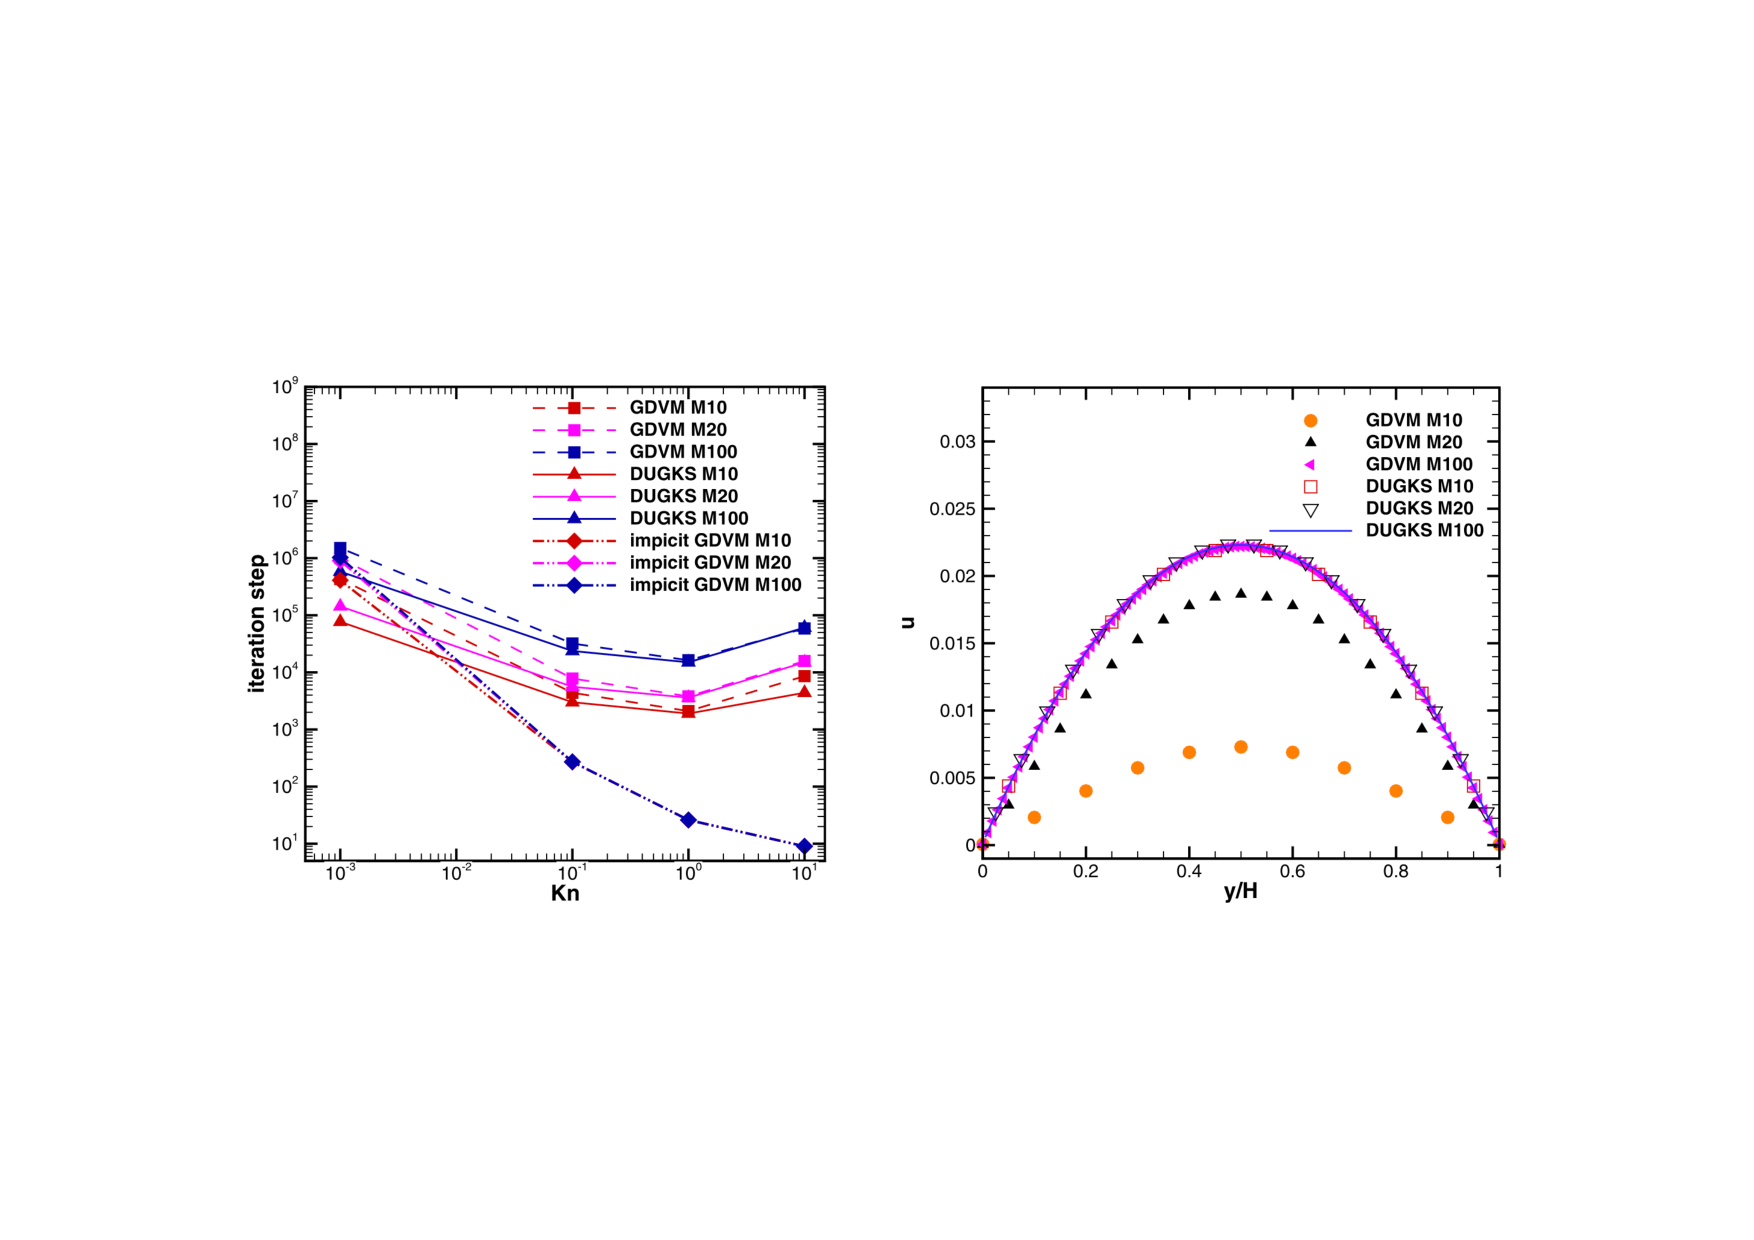
\includegraphics[scale=0.7]{GSIS/IMG/Peng_CAF}
	\caption{ (Left) The iteration number needed to find the steady-state solution of force-driven Poiseuille flow, for both the CIS and discrete UGKS~\cite{guo2013discrete}. (Right) Velocity profiles obtained at different numbers of spatial cells (M) when $\text{Kn}=0.001$, which demonstrates that the CIS is highly dissipative when the spatial resolution is not adequate~\cite{WANG201833}. \index{unified gas kinetic scheme} }
	\label{fig:Peng_CAF}
\end{figure}

We take the following linearized Shakhov model \index{kinetic model!Shakhov} to analyze the mathematical properties of CIS in the search of steady-state solutions:
\begin{equation}\label{bgkfd}
\bm{v} \cdot \bm \nabla {h^{k+1}} =\mathcal{L}_s^{+,k}- \delta_{rp}  h^{k+1}+\text{source term}, 
\end{equation}
where the gain part of the linearized collision operator is
\begin{equation}\label{LBE_Shakhov}
	\mathcal{L}^+_{s}=\delta_{rp}\left[\varrho+2\bm{u}\cdot\bm{v}+T\left(v^2-\frac{3}{2}\right)+\frac{4(1-\text{Pr})}{5}\bm{q}\cdot{\bm{v}}\left(v^2-\frac{5}{2}\right)\right]f_{eq},
\end{equation} 
and the source term is due to, e.g., the presence of pressure and temperature gradients.


Figure~\ref{fig:Peng_CAF} shows the iteration numbers needed to get the steady-state solution in the Poiseuille flow between two parallel plates. When the Knudsen number $\text{Kn}$ is large, stationary solution can be found in about 10 iterations, which means that CIS is very efficient. However, when $\text{Kn}$ is small, about one million iterations are needed, and yet the solution is contaminated by large numerical dissipation when the spatial cell size is not small enough.  

%In the following, we analyze why the slow convergence takes place.


\subsection{Slow convergence}

We adopt the Fourier stability analysis \index{Fourier stability analysis} to rigorously investigate the efficiency of CIS. We define the error functions between VDFs at two consecutive iterations as
\begin{equation}\label{Diff_Y}
Y^{k+1}(\bm{x},\bm{v}\,)=h^{k+1}(\bm{x},\bm{v}\,)-h^{k}(\bm{x},\bm{v}\,), %\label{Y_expression}
\end{equation}
and the corresponding error functions for macroscopic quantities $M=[\varrho,\bm{u}, T,\bm{q}]$ as 
\begin{equation}\label{Macro_difference}
\begin{aligned}
\Phi^{k+1}(\bm{x}\,)=M^{k+1}(\bm{x}\,)-M^{k}(\bm{x}\,)=\int{Y^{k+1}(\bm{x},\bm{v}\,)\phi(\bm{v}\,)}d\bm{v},
\end{aligned}
\end{equation}
where
\begin{equation}
\phi(\bm{v}\,)=\left[1,v_1,v_2,v_3,\frac{2}{3}v^2-1,v_1\left(v^2-\frac{5}{2}\right),v_2\left(v^2-\frac{5}{2}\right),
v_3\left(v^2-\frac{5}{2}\right)
\right].
\end{equation} 

%, see Fig.~\ref{fig:iteration_demo_errordecayrate}.

To determine how fast the error decays, we seek the eigenfunctions $\bar{Y}(\bm{v}\,)$ and $\alpha=[\alpha_\varrho,\bm\alpha_{u},  \alpha_{T},\bm\alpha_{q}]$ of the following forms:
\begin{equation}\label{an_first_satz}
\begin{aligned}[b]
Y^{k+1}(\bm{x},\bm{v}\,)=e^{k}\bar{Y}(\bm{v}\,)\exp(i\bm{\theta}\cdot{\bm{x}}\,),\\
\Phi^{k+1}(\bm{x}\,)=e^{k+1}\alpha\exp(i\bm{\theta}\cdot{\bm{x}}\,),
\end{aligned}
\end{equation}
where  $\bm{\theta}=(\theta_1,\theta_2,\theta_3)$ is the wavevector of perturbance. Note that the two exponents in the right-hand-side are different, due to the fact that in CIS we first need macroscopic quantities to start the iteration. 
The iteration is unstable when the error decay rate $e$ is larger than unity, and slow (fast) convergence occurs when the error decay rate $|e|$ approaches one (zero). %In the calculation of $e$, the convective operator in Eq.~\eqref{bgkfd} is kept intact; the convergence rate of the spatially-discretized gas kinetic equation will be shown in numerical simulations later. \index{error decay rate}

From Eqs.~\eqref{Macro_difference} and~\eqref{an_first_satz} we have 
\begin{equation}\label{relation}
e\alpha=\int \bar{Y}(\bm{v}\,)\phi(\bm{v}\,)d\bm{v},
\end{equation}
and from Eqs.~\eqref{bgkfd}, \eqref{Diff_Y}, and \eqref{an_first_satz}, we have
\begin{equation}\label{y0_solution_CIS}
\begin{aligned}[c]
\bar{Y}(\bm{v}\,)=&\frac{ \alpha_\varrho+2\bm\alpha_{u}\cdot\bm{v}+\alpha_T\left(v^2-\frac{3}{2}\right)+\frac{4(1-\text{Pr})}{5}\bm\alpha_{q}\cdot\bm{v}\left({v}^2-\frac{5}{2}\right) }{ 1+i{\delta^{-1}_{rp}}\bm{\theta}\cdot\bm{v} } {f_\text{eq}}.
\end{aligned}
\end{equation}

On multiplying Eq.~\eqref{y0_solution_CIS} with $\phi(\bm{v})$ and integrating the resultant equations with respect to $\bm{v}$, we obtain eight linear equations for eight unknown elements in $\alpha$ with the help of Eq.~\eqref{relation}:
\begin{equation}
C_8\alpha^\top=e\alpha^\top, 
\end{equation} 
where the superscript $\top$ is the transpose operator. The error decay rate is the maximum eigenvalue in magnitude of matrix $C_8$; the result\footnote{If without specification, the perturbation wavevector is chosen as $|\bm\theta|=1$; Behaviors of the error decay rate are similar for other values of $|\bm\theta|$.} is shown in Fig.~\ref{fig:SR}. Specifically, when $\text{Kn}\rightarrow0$, the error decay rate is calculated analytically~\cite{Su2020SIAM}:
\begin{equation}\label{analytical_CIS}
e_{CIS}=1-\frac{1}{2\delta^2_{rp}}.
\end{equation}

The results show that CIS is efficient in the free-molecular regime, as $e\rightarrow0$ so that the error decays quickly. On the other hand, the CIS is extremely slow in the near-continuum flow regime, as $e\rightarrow1$ when $\text{Kn}\rightarrow0$. 

\begin{figure}[t]
	\centering
%	\includegraphics[scale=0.5]{convergenceRateScheme.pdf}
	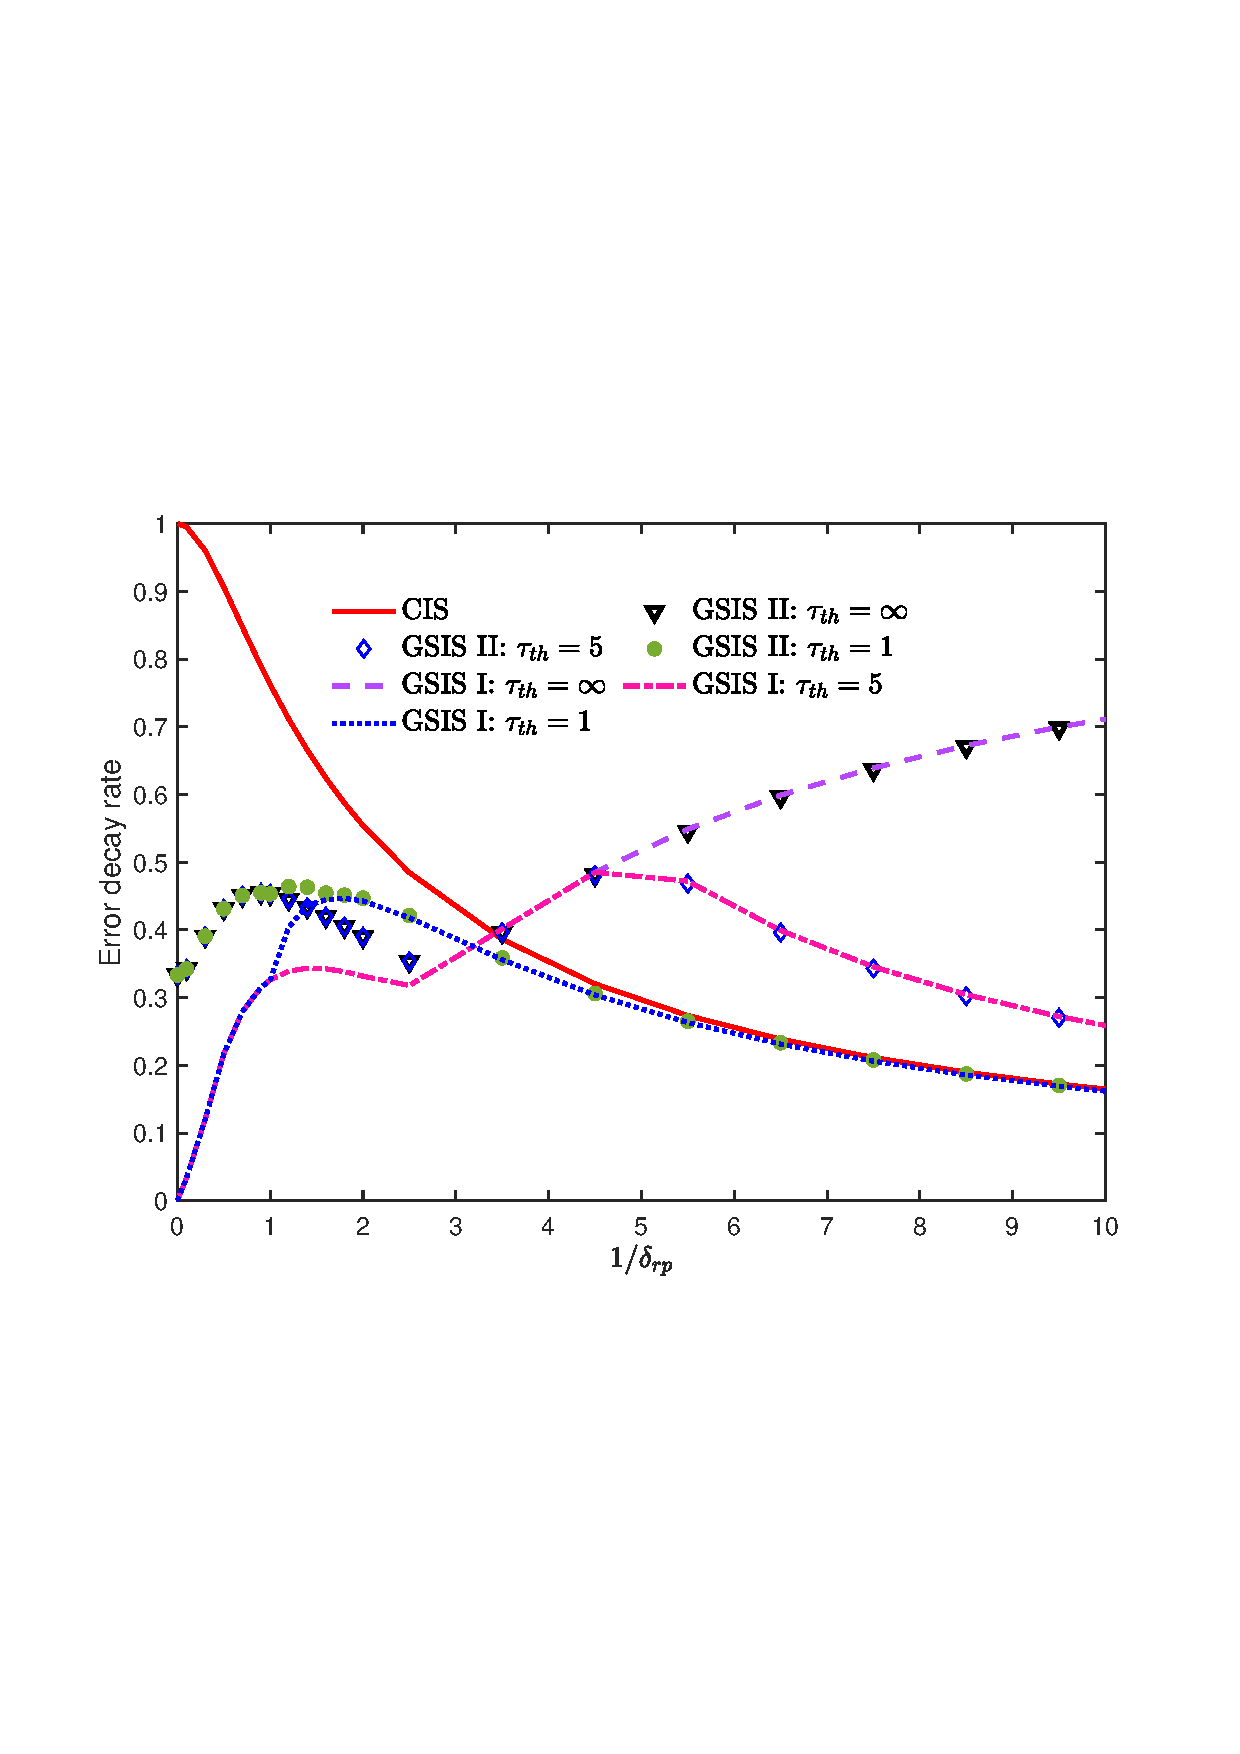
\includegraphics[width=0.7\columnwidth]{GSIS/IMG/convergenceRateScheme12.pdf}
	\caption{ 
		The error decay rate calculated from the linearized Shakhov model by the Fourier stability analysis~\cite{Su2020SIAM}. In GSIS, different threshold rarefaction parameters $\delta_{rp}^{th}$ are considered, see Eq.~\eqref{relax_parameter}. 
	}
	\label{fig:SR}
\end{figure}


\subsection{False convergence}

In addition to the slow convergence when $\text{Kn}\rightarrow0$, CIS suffers the problem of ``false convergence''. This can be analyzed following the work of Adam and Larsen for radiation transfer equation~\cite{DSA2002}. We rewrite the iterative scheme~\eqref{bgkfd} as
\begin{equation}
h^k=\mathcal{I}h^{k-1}, \quad\text{with~~}
\mathcal{I}=\frac{\mathcal{L}^+_s}{\delta_{rp}+\bm{v}\cdot\nabla}.
\end{equation}

The exact solution $h$ (the corresponding macroscopic quantities are denoted by $\Phi_M$) satisfies $h=\mathcal{I}h$. Therefore, at the $k$-th step, the difference from the exact solution is
$h-h^k=\mathcal{I}(h-h^{k-1})=\mathcal{I}(h-h^{k})+\mathcal{I}(h^k-h^{k-1})$,
so
\begin{equation}
h-h^k=\frac{\mathcal{I}}{1-\mathcal{I}}(h^k-h^{k-1}).
\end{equation}
This yields an estimation:
\begin{equation}
|h-h^k|\le\left|\frac{\mathcal{I}}{1-\mathcal{I}}\right|~ |h^k-h^{k-1}|
\approx \frac{e}{1-e}|h^k-h^{k-1}|,
\end{equation}
which implies that, if the iteration is terminated  with the convergence criterion $|\Phi_M^{k+1}-\Phi_M^{k}|<\epsilon$, the relative difference from the true steady-state solution $\Phi_M$ can be estimated as
\begin{equation}\label{false_convergence2}
|\Phi_M^{k+1}-\Phi_M|<\frac{e_{CIS}}{1-e_{CIS}}\epsilon.
\end{equation}


With Eq.~\eqref{analytical_CIS}, it is found that the error in the final step of iteration is much larger than the preassigned value $\epsilon$:
\begin{equation}\label{false_convergence_CIS}
|\Phi_M^{k+1}-\Phi_M|\rightarrow\frac{\epsilon}{\text{Kn}^2}, \quad \text{when~}\text{Kn}\rightarrow0.
\end{equation}
Therefore, false convergence \index{convergence!false} occurs if $\epsilon$ is not set small enough. 

%To reach the same convergence criterion for $|\Phi_M^{k+1}-\Phi_M|$, the total number of iterations must at least scale as $O(\text{Kn}^{-2})$.


\section{General synthetic iterative scheme}

To eliminate the deficiencies in CIS, the synthetic iterative scheme, which is initially designed for radiation transport problem~\cite{DSA2002}, is extended to solve rarefied gas flows. Success examples include the Poiseuille flow, Couette flow, thermal transpiration, and flows driven by concentration gradient~\cite{Valougeorgis:2003zr,Lihnaropoulos2007,SZALMAS20104315,NARIS2004629,NARIS2004294,Naris2005Pof,SZALMAS201691,LeiJCP2017,SU2019573}, where the flow velocity is perpendicular to the computational domain. %, e.g., in the Poiseuille flow $u_3$ varies in the $x_1$ and $x_2$ directions, while other macroscopic quantities, such as density, $u_1$ and $u_2$, and temperature are zero. % in this case, $u_3$ is governed by a diffusion equation when $\text{Kn}\rightarrow0$. If one puts the time derivative back, the macroscopic equation will be a parabolic equation, which is the key to fast convergence since the information propagation speed can be infinite, whereas in the CIS the solver can barely feel the disturbance a few MFP away. 


%Let us take the Poiseuille flow between two parallel plates in Chapter~\ref{FSM_linear_Poiseuille} as an example to sketch the major procedure of SIS. Since the flow velocity is the primary concern here, we use the linearized BGK model:
%\begin{equation}
%v_1\frac{\partial h}{\partial x_1}=
%2\delta_{rp}u_3v_3f_{eq} - \delta_{rp}h
%	-{v_3}f_{eq}.
%\end{equation}



In synthetic iterative scheme, macroscopic synthetic equation is exactly derived from the kinetic equation, which, in the limit of $\text{Kn}\rightarrow0$, becomes the diffusion equation. When the Knudsen number is not negligible, however, the macroscopic equation has an additional source term, or high-order term, which describes the rarefaction effects. The gas kinetic equation and macroscopic synthetic equation are solved on the same spatial grids in the entire domain: at each iteration, the kinetic equation provides high-order terms to the macroscopic equation, which, when solved to the steady state, is used to correct the VDF and macroscopic quantities. Since the diffusion equation is efficient in exchange the flow information, faster convergence is achieved when $\text{Kn}\rightarrow0$. 



Synthetic equations should be carefully designed when the general rarefied gas flow is concerned. For generality  we consider the LBE. We multiply Eq.~\eqref{Chapter1_Boltzmann_lin}  by the five fundamental collision invariants and integrate the resultant equations with respect to the molecular velocity $\bm{v}$, yielding: 
\begin{equation}\label{eq123}
\begin{aligned}
\frac{\partial {\varrho}}{\partial{t}}+\frac{\partial {u_i}}{\partial{x_i}}=0, \\
2\frac{\partial {u_i}}{\partial{t}}+\frac{\partial {\varrho}}{\partial{x_i}}+\frac{\partial {T}}{\partial{x_i}}+\frac{\partial {{\sigma_{ij}}}}{\partial{x_j}}=0, \\
\frac{3}{2}\frac{\partial {T}}{\partial{t}}+\frac{\partial {{q_j}}}{\partial{x_j}}+\frac{\partial {u_j}}{\partial{x_j}}=0.
\end{aligned}
\end{equation}


%One way to close Eq.~\eqref{eq123} is to use the Chapman-Enskog expansion. 
%When the VDF is truncated at the first-order of $\mathrm{Kn}$, i.e., $
%h=\mathrm{Kn} h^{(1)}$,
%we have 
%\begin{equation}\label{GTMNSF}
%\begin{aligned}[b]
%\sigma_{ij} =-\delta_{rp}^{-1}\left(\frac{\partial u_{i}}{\partial x_{j}}+\frac{\partial u_{j}}{\partial x_{i}}-\frac{2}{3}\frac{\partial u_{k}}{\partial x_{k}}\delta_{ij}\right)\equiv-2\delta_{rp}^{-1}\frac{\partial u_{<i}}{\partial {x_{j>}}}, \\
%q_i = -\frac{5}{4\mathrm{Pr}}\delta_{rp}^{-1} \frac{\partial T}{\partial x_i},
%\end{aligned}
%\end{equation}
%and Eq.~\eqref{eq123} reduces to the linearized NSF equations. Higher-order macroscopic equations can be obtained successively via the Chapman-Enskog expansion but they are not stable. On the other hand, even the obtained high-order macroscopic equations are stable, they are only approximate solutions of the Boltzmann equation, rather than  exact. Therefore, they cannot describe the RGD in the entire flow regimes.


%It should be noted that in the implicit UGKS~\cite{zhuyajun2016} and other variants~\cite{yang2018PoF,yang2018PRE}, both the gas kinetic equation and  macroscopic equations are solved, where $\sigma_{ij}$ and $\bm{q}$ are directly calculated from the VDF. These methods are efficient when the Knudsen number is large, like the CIS. However, in the near-continuum flow regime, the number of iterations are still large, at the order of thousands iterations. The reason for the relative slow convergence is that, if the iteration starts from the global equilibrium state where $\sigma_{ij}$ and $\bm{q}$ are zero, in most of the time the Euler equations, rather than the NSF equations that dominates the steady-state flow dynamics, are solved, due to the fact that perturbance from the wall takes a long time to reach the bulk region in near-continuum flows. This is a physical problem, and any numerical scheme cannot be used to find the steady-state solution efficiently if the underlying physics is not properly taken into account.	


%Even when the shear stress and heat flux are non-zero, solutions of Eq.~\eqref{eq123} deviate from that of the Navier-Stokes equations in the near-continuum flow regime unless they nearly converge to the steady-state solutions. As a matter of fact, the authors have checked, in the linearized Poiseuille flow~\cite{LeiJCP2017}, that when the kinetic equations is solved by CIS, Eq.~\eqref{eq123} cannot help to find converged solution within dozens of iterations. 


To develop a general fast-converging scheme, it is beneficial to construct macroscopic diffusion-type equations that contain Newton's law for stress and Fourier's law for heat conduction explicitly to recover the macroscopic transport mechanism; we express the shear stress and heat flux as follows:
\begin{eqnarray}
\sigma_{ij} =-2\delta_{rp}^{-1}\frac{\partial u_{<i}}{\partial {x_{j>}}}+\text{HoT}_{\sigma_{ij}}, \label{sigma_first_HoT}\\
q_i =-\frac{5}{4\mathrm{Pr}}\delta_{rp}^{-1} \frac{\partial T}{\partial x_i}+\text{HoT}_{q_i}, \label{q_first_HoT}
\end{eqnarray}
where $\text{HoT}_{\sigma_{ij}}$ and $\text{HoT}_{q_i}$ are the high-order terms containing contributions of all the orders $O(\text{Kn}^\alpha)$ with $\alpha=2,3,\cdots,\infty$.
\index{constitutive relation}
These high-order terms cannot be obtained from Burnett, super-Burnett equations, nor from the Grad moment equations, but have to be determined from the kinetic equation that are valid in the whole range of rarefaction.  


\subsection{Scheme-I GSIS}

To obtain Eq.~\eqref{sigma_first_HoT}, we multiply Eq.~\eqref{Chapter1_Boltzmann_lin} by $2v_{<i}v_{j>}$ and integrate the resultant equation with respect to $\bm{v}$:
\begin{equation}\label{HoT_sigma0}
\begin{aligned}[b]
\frac{\partial \sigma_{ij}}{\partial {t}}
+2\int{v_{<i}v_{j>}} \bm{v}\cdot\frac{\partial h}{\partial \bm{x}}d\bm{v} =2\int{\mathcal{L}v_iv_j}\mathrm{d}\bm{v},
\end{aligned}
\end{equation}
which is rewritten as
\begin{equation}\label{HoT_sigma}
\begin{aligned}[b]
\frac{\partial \sigma_{ij}}{\partial {t}}
&+\underbrace{2\int{v_{<i}v_{j>}} \bm{v}\cdot\frac{\partial h}{\partial \bm{x}}d\bm{v}-2\frac{\partial{u_{<i}}}{\partial {x_{j>}}}}_{\text{HoT}_{\sigma_{ij}}}\\
&+\underbrace{2\frac{\partial{u_{<i}}}{\partial {x_{j>}}}=-\delta_{rp}\sigma_{ij}}_{\text{Newton's law}}+2\int{(\mathcal{L}-\mathcal{L}_s)v_iv_j}\mathrm{d}\bm{v}.
\end{aligned}
\end{equation}

Note that the purpose of introducing $\mathcal{L}_s$ is only to produce the term $\delta_{rp}\sigma_{ij}$, so that the Newton law appears in the synthetic equation naturally; this turns out to be crucial in boosting convergence. Also note that, for the linearized BCO, comparing to $\delta_{rp}\sigma_{ij}$, the term $2\int{(\mathcal{L}-\mathcal{L}_s)v_iv_j} d\bm{v}$ is negligible. For instances,  this term is zero for Maxwell gas, while for the HS gas this term is only about 2\% of $\delta_{rp}\sigma_{ij}$, see Eq.~\eqref{transport_high_oder}. It will be shown later that the high-order terms is evaluated at the $k$-th iteration step, while Newton's law for stress is calculated at the $(k+1)$-th step. \index{Newton's law of stress}






Similarly, to obtain Eq.~\eqref{q_first_HoT}, we multiply Eq.~\eqref{Chapter1_Boltzmann_lin} by $v_i(v^2-5/2)$ and integrate the resultant equation with respect to $\bm{v}$:
\begin{equation}\label{HoT_q}
\begin{aligned}
\frac{\partial q_{i}}{\partial {t}}
&+\underbrace{ \int{\left(v^2-\frac{5}{2}\right)}v_i \bm{v}\cdot\frac{\partial h}{\partial \bm{x}}d\bm{v}
		-\frac{3C_q}{2}\frac{\partial{T}}{\partial {x_{i}}
} }_{\text{HoT}_{q_i}} \\
&+\underbrace{\frac{3C_q}{2}\frac{\partial{T}}{\partial {x_{i}}}=-\delta_{rp}\text{Pr}q_{i}}_{\text{ Fourier's law}}+\int{(\mathcal{L}-\mathcal{L}_s)v_iv^2} \mathrm{d}\bm{v}.
\end{aligned}
\end{equation}
For the linearized BCO, the term $\int{(\mathcal{L}-\mathcal{L}_s)v_iv^2} d\bm{v}$ is negligible small when compared to $\delta_{rp}q_{i}$. If we choose $C_q=5/6$, Fourier's heat conduction law appears naturally. \index{Fourier's law of heat conduction}


%It is noted that the synthetic equations~\eqref{eq123}, \eqref{HoT_sigma} and \eqref{HoT_q} resemble the Grad 13 moment \index{moment equations!Grad 13} equations~\cite{Grad1949,henning}. However, since the higher-order terms are computed directly from the VDF, no approximations are introduced. %If the VDF is approximated by Gauss-Hermite polynomials to the third order, where the coefficients before those polynomials are determined by the first 13 moments of  VDF, then the G13 moment equations will be recovered.  
%Since the first-order Chapman-Enskog expansion to G13 equations leads to Eqs.~\eqref{eq123} and~\eqref{GTMNSF}, that is, only the underlined terms in Eqs.~\eqref{HoT_sigma} and~\eqref{HoT_q} are retained~\cite{henning}, the synthetic equations~\eqref{eq123}, \eqref{HoT_sigma} and~\eqref{HoT_q} asymptotically preserve the NSF limit, which we will prove rigorously later. Thus, they should be able to boost the convergence to  steady-state solutions of the LBE significantly, as in the bulk region (a few molecular MFP away from solid surfaces) we are effectively solving the NSF equations, the limiting equation of the LBE with diffusion operators for velocity and temperature.


The GSIS is designed to find steady-state solutions of the LBE through the following steps~\eqref{Chapter1_Boltzmann_lin}:
\begin{itemize}
	\item Step 1. When the VDF $h^{k}$ and the corresponding macroscopic quantities are known,  calculate $2\int{(\mathcal{L}-\mathcal{L}_s)v_iv_j}\mathrm{d}\bm{v}$  and $\int{(\mathcal{L}-\mathcal{L}_s)v_iv^2}\mathrm{d}\bm{v}$. Also calculate the VDF $h^{k+1/2}$ at the intermediate iterative step  as: 
	\begin{equation}\label{syn_LBE0}
	\nu_{eq}(\bm{v})h^{k+1/2}+\bm{v}\cdot\frac{\partial
		{h}^{k+1/2}}{\partial{\bm{x}}}=\mathcal{L}^+(h^{k},f_{eq}).
	\end{equation}

	\item Step 2. From $h^{k+1/2}$, calculate the macroscopic quantities at the intermediate step, and the high-order terms.
	
	\item Step 3. Calculate the macroscopic quantities, in the bulk region, at the $(k+1)$-th step by solving synthetic equations~\eqref{eq123}, \eqref{HoT_sigma} and \eqref{HoT_q} to the steady state, where the boundary conditions in the vicinity of walls are obtained from Step 2.
	
	%That is, for steady-state problems the stress and heat flux can be obtained from Eq.~\eqref{HoT_sigma} and~\eqref{HoT_q}, which will then be substituted to Eq.~\eqref{eq123} to form the NSF equations with source terms from  higher-order terms. These equation can be solved by the SIMPLE algorithm or DG method easily in the bulk region, where the boundary conditions in the vicinity of walls for density, velocity, temperature are obtained from Step 2. 
	%The detailed DG algorithm to solve the synthetic equations can be found in the Appendix~\ref{appen_HDG}.
	
	
	\item  Step 4. The VDF is corrected in the following manner so that its corresponding macroscopic quantities is the same as those obtained in Step 3:
	\begin{equation}\label{guided0}
	\begin{aligned}[b]
	h^{k+1}=&h^{k+1/2}+\left[\lambda_{\rho}
	+2\lambda_{\bm{u}}\cdot{\bm{v}}+\lambda_T\left(v^2-\frac{3}{2}\right)
\right]f_{eq}\\
	+&\left[
	\lambda_{\sigma_{ij}}\left(v_iv_j-\frac{v^2}{3}\delta_{ij}\right)
	+\frac{4}{5}{\lambda_q}\cdot\bm{v}\left(v^2-\frac{5}{2}\right)
		\right]f_{eq},
	\end{aligned}
	\end{equation}
	where $\lambda_{\bm{u}}=\bm{u}^{k+1}-\bm{u}^{k+1/2}$, $\lambda_{\bm{q}}=\bm{q}^{k+1}-\bm{q}^{k+1/2}$, $\lambda_{\rho}=\rho^{k+1}-\rho^{k+1/2}$,  $\lambda_T=T^{k+1}-T^{k+1/2}$, and $\lambda_{\sigma_{ij}}=\sigma_{ij}^{k+1}-\sigma_{ij}^{k+1/2}$.
	
	\item Step 5. The above steps are repeated until convergence.
\end{itemize}



%Since the gas kinetic equation is solved together with the macroscopic equations~\eqref{eq123}, \eqref{HoT_sigma} and~\eqref{HoT_q} for general rarefied gas flows, the above scheme is called general synthetic iterative scheme (GSIS). 

%Note that although the SIS has been widely applied to the radiation transport processes~\cite{DSA2002} and rarefied gas flows driven by local pressure, temperature, and concentration gradients~\cite{Valougeorgis:2003zr,Naris2005Pof,CircularSIS2013,szalmas2010,WeiSuJCP1} to overcome the slow convergence and remove the constraint on the spatial cell size in the near-continuum flow regime, it is the first time that the GSIS is developed for general rarefied gas flows described by the LBE.  Also, it is with no doubt that such a methodology can be directly applied to construct the GSIS for the nonlinear Boltzmann equation.


\subsection{Scheme-II GSIS}

High-order terms in Eqs.~\eqref{HoT_sigma} and~\eqref{HoT_q} are constructed by considering the evolution equation of stress and heat flux, which involves the calculation of complicated collision operator when the Boltzmann equation is considered. This is not a problem for deterministic numerical methods, but will be not easy for DSMC. \index{DSMC}
As we aim to develop a generalized scheme, not only for deterministic methods, but also for stochastic methods such as DSMC, we propose the following easy-to-use constitutive relations~\cite{Zhu2021JCP}: \index{constitutive relation}
\begin{equation}\label{hotdiffint}
\begin{aligned}[b]
\text{HoT}_{\sigma_{ij}} = \sigma^{k+1/2}_{ij} +2\delta_{rp}^{-1}\frac{\partial u^{k+1/2}_{<i}}{\partial {x_{j>}}},\\
\text{HoT}_{q_i} = q_i^{k+1/2} +\frac{5}{4\mathrm{Pr}}\delta_{rp}^{-1} \frac{\partial T^{k+1/2}}{\partial x_i}.
\end{aligned}
\end{equation}
%This will be called Scheme II in the following book, while these in Eqs.~\eqref{HoT_sigma} and~\eqref{HoT_q} will be called Scheme I. 


%The scheme I is more complicated than the scheme II, because (i) it involves the calculation of BCO  and (ii) the underline terms in Eqs.~\eqref{HoT_sigma} and~\eqref{HoT_q} contain spatial derivations which may lead to numerical instabilities around sharp solid corners. Therefore, if both schemes have  similar capability in boosting convergence,  the scheme II will be preferred. In addition, the scheme II can be directly applied to solve the gas kinetic equations involving multi-species and chemical reactions, where the scheme I will be extremely complicated.






\section{Properties of GSIS}\label{secIII}

Two important questions in the multiscale simulation of rarefied gas flows are: can we find the steady-state efficiently and can we get accurate results even at coarse spatial grid? This section is dedicated to proving both. 

\subsection{Super convergence}
\index{convergence!super}

The linearized Shakhov model is used to analyze the error decay rate of GSIS. That of the Boltzmann equation can only be shown in numerical simulation, due to the complicated structure of the BCO.  

The error functions in Eqs.~\eqref{Diff_Y}, \eqref{Macro_difference}, and \eqref{an_first_satz} are redefined as
\begin{equation}\label{Y_ansatz2} 
\begin{aligned}[b]
Y^{k+1/2}(\bm{x},\bm{{v}}\,)=h^{k+1/2}(\bm{x},\bm{{v}}\,)-h^{k}(\bm{x},\bm{{v}}\,)=e^{k}\bar{Y}(\bm{{v}}\,)\exp(i\bm{\theta}\cdot{\bm{x}}\,),\\
\Phi^{k+1}(\bm{x}\,)=M^{k+1}(\bm{x}\,)-M^{k}(\bm{x}\,)=e^{k+1}\alpha\exp(i\bm{\theta}\cdot{\bm{x}}\,),
\end{aligned}
\end{equation}
where $\bar{Y}(\bm{{v}}\,)$ is still given by Eq.~\eqref{y0_solution_CIS}. Note that now $\Phi$ are calculated from the synthetic equations, rather than from the VDF. \index{Fourier stability analysis}
That is, macroscopic quantities at the $(k+1)$-th iteration step are obtained by solving the following synthetic equations:
\begin{equation}\label{eq123_lin}
\begin{aligned}[b]
\frac{\partial {u^{k+1}_i}}{\partial{x_i}}=0,\quad
\frac{\partial {\varrho^{k+1}}}{\partial{x_i}}+\frac{\partial {T^{k+1}}}{\partial{x_i}}+\frac{\partial {{\sigma^{k+1}_{ij}}}}{\partial{x_j}}=0, \quad
\frac{\partial {{q^{k+1}_{i}}}}{\partial{x_i}}=0.	
\end{aligned}
\end{equation}


With Eqs.~\eqref{y0_solution_CIS},  \eqref{HoT_sigma}, \eqref{HoT_q}, \eqref{eq123_lin}, and~\eqref{Y_ansatz2}, we obtain the following eight linear equations: \index{error decay rate}
\begin{equation}\label{L_lin1}
\begin{aligned}[b]
e(i\theta_1\alpha_{u_1}+i\theta_2\alpha_{u_2}+i\theta_3\alpha_{u_3})=0, \\
e[i\theta_j(\alpha_\varrho+\alpha_T)+|\bm{\theta}|^2{\delta^{-1}_{rp}}\alpha_{u_j}]=S_{j+1},\\
e(i\theta_1\alpha_{q_1}+i\theta_2\alpha_{q_2}+i\theta_3\alpha_{q_3})=0,\\
e\left(\frac{5i}{4\text{Pr}}\theta_j{\delta^{-1}_{rp}}\alpha_{T}+\alpha_{q_j}\right)=S_{j+5},
\end{aligned}
\end{equation}
where $j=1,2,3$, and the source terms in the scheme I, due to the HoTs in Eqs.~\eqref{HoT_sigma} and~\eqref{HoT_q}, are also linear functions of $\alpha_M$:
\begin{equation}\label{L_lin2}
\begin{aligned}[b]
S_{j+1}=\delta^{-1}_{rp}\int\left(|\bm{\theta}|^2{v}_j-2\Theta
\theta_kv_{<j}v_{k>}\right)\bar{Y}(\bm{{v}}\,)\mathrm{d}^3\bm{{v}}, \\
%S_3=\delta^{-1}_{rp}\int\left[|\bm{\theta}|^2{v}_2-2\Theta (\theta_1{v}_1 {v}_2+\theta_2v_{<2}v_{2>}+\theta_3{v}_2 {v}_3)\right]\bar{Y}(\bm{{v}}\,)\mathrm{d}^3\bm{{v}}, \\
%S_4=\delta^{-1}_{rp}\int\left[|\bm{\theta}|^2{v}_3-2\Theta (\theta_1{v}_1 {v}_3+\theta_2{v}_2 {v}_3+\theta_3v_{<3}v_{3>})\right]\bar{Y}(\bm{{v}}\,)\mathrm{d}^3\bm{{v}}, \\
S_{j+5}=\frac{i}{\delta_{rp}\text{Pr}}\int\left[\frac{5}{4\text{Pr}}\theta_j\left(\frac{2}{3}{v}^2-1\right)-\Theta{v}_j\left({v}^2-\frac{5}{2}\right)\right]\bar{Y}(\bm{{v}}\,)\mathrm{d}^3\bm{{v}},
\end{aligned} 
\end{equation} 
where $\Theta=\theta_1{v}_1+\theta_2v_2+\theta_3v_3$, $k=1,2,3$ is the dummy index, while that in the scheme II, with Eq.~\eqref{hotdiffint}, are
\begin{equation}\label{L_lin_shcemeII}
\begin{aligned}[b]
S_{j+1}=\int\left({\delta^{-1}_{rp}}{}|\bm{\theta}|^2{v}_j-2i\theta_kv_{<j}v_{k>}\right)\bar{Y}(\bm{{v}}\,)\mathrm{d}^3\bm{{v}}, \\
%S_3=\int\left[{\delta^{-1}_{rp}}{}|\bm{\theta}|^2{v}_2-2i\theta_2v_{<2}v_{2>}-2i\theta_1{v}_1{v}_2-2i\theta_3{v}_2{v}_3\right]\bar{Y}(\bm{{v}}\,)\mathrm{d}^3\bm{{v}}, \\
%S_4=\int\left[{\delta^{-1}_{rp}}{}|\bm{\theta}|^2{v}_3-2i\theta_3v_{<3}v_{3>}-2i\theta_1{v}_1{v}_3-2i\theta_2{v}_2{v}_3\right]\bar{Y}(\bm{{v}}\,)\mathrm{d}^3\bm{{v}}, \\
S_{j+5}=\int\left[\frac{5i}{4\text{Pr}}\theta_j{\delta^{-1}_{rp}}{}\left(\frac{2}{3}{v}^2-1\right)+{v}_j\left({v}^2-\frac{5}{2}\right)\right]\bar{Y}(\bm{{v}}\,)\mathrm{d}^3\bm{{v}},
%\\
%S_7=\int\left[\frac{5}{4\text{Pr}}i\theta_2{\delta^{-1}_{rp}}{}\left(\frac{2}{3}{v}^2-1\right)+{v}_2\left({v}^2-\frac{5}{2}\right)\right]\bar{Y}(\bm{{v}}\,)\mathrm{d}^3\bm{{v}},\\
%S_8=\int\left[\frac{5}{4\text{Pr}}i\theta_3{\delta^{-1}_{rp}}{}\left(\frac{2}{3}{v}^2-1\right)+{v}_3\left({v}^2-\frac{5}{2}\right)\right]\bar{Y}(\bm{{v}}\,)\mathrm{d}^3\bm{{v}}.
\end{aligned} 
\end{equation}


For the scheme I, the error decay rate is obtained by solving Eqs.~\eqref{L_lin1} and~\eqref{L_lin2}, which  are rewritten in the matrix form as
\begin{equation}
L_8e\alpha^\top=R_8\alpha^\top,
\end{equation}
where $L_8$ and $R_8$ are two $8\times8$ matrices. By introducing $G_1=L_8^{-1}R_8$ and numerically computing its eigenvalues we obtain the error decay rate $e$ in Fig.~\ref{fig:SR}. When $\text{Kn}\rightarrow0$, that is, $e\propto \text{Kn}^2$, so GSIS can boost convergence in near-continuum flows. As a matter of fact, compared to the false convergence of CIS described by Eq.~\eqref{false_convergence_CIS}, GSIS possesses the properties of super convergence, since according to the following equation
\begin{equation}\label{super_convergence}
|\Phi_M^{k+1}-\Phi_M|\rightarrow{\epsilon}{\text{Kn}^2}, \quad \text{when~}\text{Kn}\rightarrow0,
\end{equation}
the convergence criterion $\epsilon$ can be set at a relative larger value. \index{super convergence}

When $\text{Kn}\rightarrow\infty$, however, $e\rightarrow1$. To fix this problem, macroscopic quantities are updated as
\begin{equation}\label{GSIS_K3}
M^{k+1}(\bm{x}\,)=\beta{}M_{\text{syn}}(\bm{x})+(1-\beta)M^{k+1/2}(\bm{x}),
\end{equation}
where the parameter $\beta$ is chosen as
\begin{equation}\label{relax_parameter}
\beta=\frac{\delta_{rp}}{\text{max}(\delta_{rp},\delta_{rp}^\text{th})}.
\end{equation}
with $\delta_{rp}^\text{th}$ being the threshold rarefaction parameter. That is, $\beta=1$ when the rarefaction parameter is larger than $\delta_{rp}^\text{th}$; when $\delta_{rp}<\delta_{rp}^\text{th}$, $\beta$ gradually decreases to zero as the Knudsen number approaches infinity. The error decay rate is obtained by computing the eigenvalue of the matrix
$G=\beta{L_8^{-1}R_8}+(1-\beta)C_8$.

Results in Fig.~\ref{fig:SR} show that the maximum error decay rate can be restrained to be less than 0.5 for all Knudsen number, by choosing approximate value of $\beta$.  Thus, theoretically, GSIS can achieve fast convergence in the whole range of Knudsen number, because  the error is reduced by three orders of magnitude in 10 iterations. 


Likewise, for the scheme II, the error decay rate is obtained by solving Eqs.~\eqref{L_lin1} and~\eqref{L_lin_shcemeII}.  It is seen from Fig.~\ref{fig:SR} that when $\text{Kn}\rightarrow0$, the error decay rate of the scheme II is reduced from one in CIS, but does not goes to zero\footnote{This is because the heat flux enters the collision term in the Shakhov model, and in the Scheme II the evolution equation~\eqref{HoT_q} of heat flux is not considered in the macroscopic synthetic equation. If we use the linearized BGK model, we find that the error decay rate approaches zero when $\text{Kn}\rightarrow0$.}. Nevertheless, like the scheme I, by choosing appropriate value of $\delta_{rp}^{th}$, the error decay rate can also be controlled within 0.5 in the whole range of rarefaction parameter.
	
	

%Note that the Fourier stability analysis is conducted in spatial periodic system. In reality, however, solid walls are always present, and the Knudsen layer (exists in a region within a few MFP away from the wall, see Chapter~\ref{chap:velocity_slip}) makes the effective Knudsen number $\text{Kn}\sim1$. Therefore, the maximum error decay rate in the whole range of Knudsen number is a more important indicator of efficiency. In this sense, from Fig.~\ref{fig:SR} we see that both GSIS schemes have similar efficacy in boosting the convergence to steady-state solutions. We therefore recommend the scheme II over scheme I because it is simpler and can be easily applied to other BCOs.
	


%
%\subsubsection{Importance of NSF constitutive relations}\label{sec:whyimportant}
%
%Note that when the Knudsen number is small, we choose $\beta=1$ in Eq.~\eqref{relax_parameter} and $C_q=5/6$ in Eq.~\eqref{HoT_q}; this means that in the near-continuum regime, the constitutive relations in the NSF equations, i.e., Newton's law for shear stress and Fourier's law for heat conduction, are explicitly included in the synthetic equations. This turns out to be extremely important for the fast convergence of GSIS, as the error decay rate goes to zero when $\text{Kn}\rightarrow0$.
%
%
%\begin{figure}[t]
%	\centering
%	\includegraphics[scale=0.45]{GSIS/IMG/Why_NSF.pdf}
%	\caption{The error decay rate as a function of the rarefaction parameter in the scheme I of GSIS, when $C_q$ in Eq.~\eqref{HoT_q} takes different values. }
%	\label{fig:whyimportant}
%\end{figure}
%
%To demonstrate this superiority, we calculate the error decay rate $e$ by choosing different values of $C_q$ when the Knudsen number $K$ is small; the results in Fig.~\ref{fig:whyimportant} show that only when $C_q=5/6$ can the error decay rate approaches zero when $K\rightarrow0$. Moreover, when $\text{Kn}<0.2$, the further  $C_q$ deviates away from $5/6$, the larger the error decay rate and hence the slower the convergence. When $C_q$ deviates too much from $5/6$, say $C_q=1/3$, $e$ can be even larger than one, which means that the iteration is unstable. 
%
%
%These results confirm that the fastest convergence can be realized by including the NSF constitutive relations explicitly in synthetic equations. The secret to the fast convergence of GSIS is that Eqs.~\eqref{eq123}, \eqref{HoT_sigma} and~\eqref{HoT_q} are exactly the linearized NSF equations of the corresponding kinetic equation when higher-order terms are neglected, which lead to diffusion equations for the flow velocity and temperature; these diffusion equations enable efficient flow information exchange across the whole computational domain. 


%\leir{If the heat flux in Eq.~\eqref{HoT_q} is directly computed from the $h^{k+1/2}$, i.e. by setting $C_q=0$ according to Eqs.~\eqref{NS_shear_def} and~\eqref{NS_heat_def}, there are no diffusion equations for the velocity and temperature. }


\subsection{Asymptotic preserving}\label{asymptotic_preserving}
\index{asymptotic preserving}

In GSIS the mesoscopic kinetic equation and macroscopic synthetic equations can be solved by different numerical methods with different order of accuracy. It is important to investigate the influence of spatial discretization of the gas kinetic solver on the accuracy of GSIS, based on the assumptions that (i) synthetic equations can be solved exactly and (ii) the spatial cell size $\Delta{x}$ is adequate to capture the physical solution of NSF equations. This is equivalent to check whether the NSF equations can be exactly derived or not, through the \index{Chapman-Enskog expansion} Chapman-Enskog expansion~\cite{CE}, from the discretized gas kinetic equation 
\begin{equation}\label{LBE_first_GSIS}
\bm{v}\cdot\frac{\partial{h}}{\partial\bm{x}}+O(\Delta{x}^n)\delta(h)=\mathcal{L}_s - \delta_{rp}  h,
\end{equation}
with the following scaling ($\Delta{x}$ has been normalized by the characteristic flow length $L$):
\begin{equation}\label{scaling}
\Delta{x}\sim{\text{Kn}^{1/\alpha}},
\end{equation}
where $n$ is the order of approximation for the spatial derivative,  $\delta(h)$ is the $(n+1)$-th order derivative of $h$, and $\alpha$ is order of accuracy in the asymptotic preserving of NSF equations.  


%Since in GSIS the mass, velocity and temperature are obtained from solving Eqs.~\eqref{macro_1} to~\eqref{higher_order_app2}, we find that if we have $h_0=h_{eq}$, the synthetic equations are reduced to the linearized Navier-Stokes equation exactly.


\subsubsection{Scheme I}



By subsisting the expansion $h=h_0+\text{Kn}h_1+\cdots$ into Eq.~\eqref{LBE_first_GSIS} and collecting terms with the order of $\text{Kn}^{-1}$, we have $h_0=f_{eq}$, when the following largest scaling is chosen
\begin{equation}\label{scaling1}
\Delta{x}\sim{\text{Kn}^{1/\infty}}=O(1).
\end{equation}
Under this scaling, at the order $\text{Kn}^{0}$, we obtain:
\begin{equation}
h_1=-\bm{v}\cdot\frac{\partial{h_{eq}}}{\partial\bm{x}}-\delta(h_{eq}).
\end{equation}
 Thus, according to Eqs.~\eqref{HoT_sigma} and~\eqref{HoT_q},  the linear constitutive relations are recovered in synthetic equations with accuracy $O(\text{Kn}^2)$:
\begin{equation}\label{NSF_relations}
\begin{aligned}[b]
\sigma_{ij} =-2\delta_{rp}^{-1}\frac{\partial u_{<i}}{\partial {x_{j>}}}
+O(\text{Kn}^2), \\
q_i =-\frac{5}{4\text{Pr}}\delta_{rp}^{-1}\frac{\partial T}{\partial x_i}
+O(\text{Kn}^2).
\end{aligned}
\end{equation} 





Thus, GSIS asymptotically preserves the NSF equations, provided that the spatial resolution $\Delta{x}=O(1)$ is able to capture the physical solution of NSF equations.  In practice, however, $\Delta{x}=O(1)$ cannot be used in regions where the physical solutions require a resolution of $O(\text{Kn})$, e.g., the  Knudsen layer and shock structure. Fortunately, these kinetic layers only occupy a small fraction of the computational domain, which can be captured by implicit schemes with non-uniform spatial discretization. 

%This will be tested in the following numerical examples.






 


\subsubsection{Scheme II}

In order to recover the NSF constitutive relations~\eqref{NSF_relations}, the VDF to the first order of Knudsen number must be exactly recovered as
\begin{equation}
h_1=-\bm{v}\cdot\frac{\partial{h_{eq}}}{\partial\bm{x}}.
\end{equation}
And this requires the following largest scaling:
\begin{equation}\label{scaling2}
\Delta{x}\sim{\text{Kn}^{1/2}}.
\end{equation}


%The asymptotic path to the limiting hydrodynamic flow regimes are summarized in Fig.~\ref{fig:GSIS_UP}. Note that both GSIS schemes can be extended to time-dependent problems~\cite{Wu2021Arxiv}, and the property of asymptotic preserving in the temporal domain is the same as the spatial domain. 


\section{Numerical tests} \label{sec:results1}

Several numerical simulations are carried out to demonstrate the major properties of GSIS, including the 1D coherent Rayleigh-Brillouin scattering problem where the influence of gas-surface interaction is absent, the planar Fourier flow, and 2D Couette flow between two non-coaxial cylinders. More challenging numerical examples can be found in Refs.~\cite{SuArXiv2019, Su2020SIAM, Su2021CMAME, Su2020CAF, Zhu2021JCP}.



\subsection{Coherent Rayleigh-Brillouin scattering} 

This problem is ideal to show the fast-converging and asymptotic-preserving properties of the GSIS, as well as the flexibility, importance, and advantage of GSIS that the kinetic and synthetic equations are solved by different methods with different order of accuracy. 

The theory of coherent RBS is elaborated in Chapter~\ref{chap:fluctuation}. Here we directly write the evolution equation for the perturbed VDF as 
\begin{equation}\label{CRBS_govering}
2\pi{i}f_sh+v_2\frac{\partial{h}}{\partial{x_2}}=\mathcal{L}_s^{+,k}-\delta_{rp}h+2v_2\cos(2\pi{x_2}),
\end{equation}
where the normalized scattering frequency is chosen as $f_s=\sqrt{5/6}$ and the last term presents the external acceleration generated by the optical lattice. The problem is spatially periodic, with the influence of gas-surface interaction. The presence of the first term in Eq.~\eqref{CRBS_govering} is due to the temporal periodicity. Correspondingly, the time derivative $\partial/\partial t$ in the synthetic equations should be replaced by $2\pi{i}f_s$.
%Note that, after obtaining $h^{(k+1/2)}$ from the kinetic equation and $\bar{M}$ from the synthetic equations, GSIS updates $h^{(k+1)}$ by the following formula:
%\begin{equation}
%\begin{aligned}
%h^{(k+1)}=h^{(k+1/2)}+\beta\bigg[ \left(\bar{\varrho}-\varrho^{(k+1/2)}\right) & +2\left(\bar{\bm{u}}-\bm{u}^{(k+1/2)}\right)\cdot\bm{v} \\
%&+\left( \bar{\tau}-\tau^{(k+1/2)} \right) \left( v^2-\frac{3}{2} \right) \bigg],
%\end{aligned}
%\end{equation}
%such that Eq.~\eqref{GSIS_K30} holds.


\begin{figure}[pt]
	\centering
	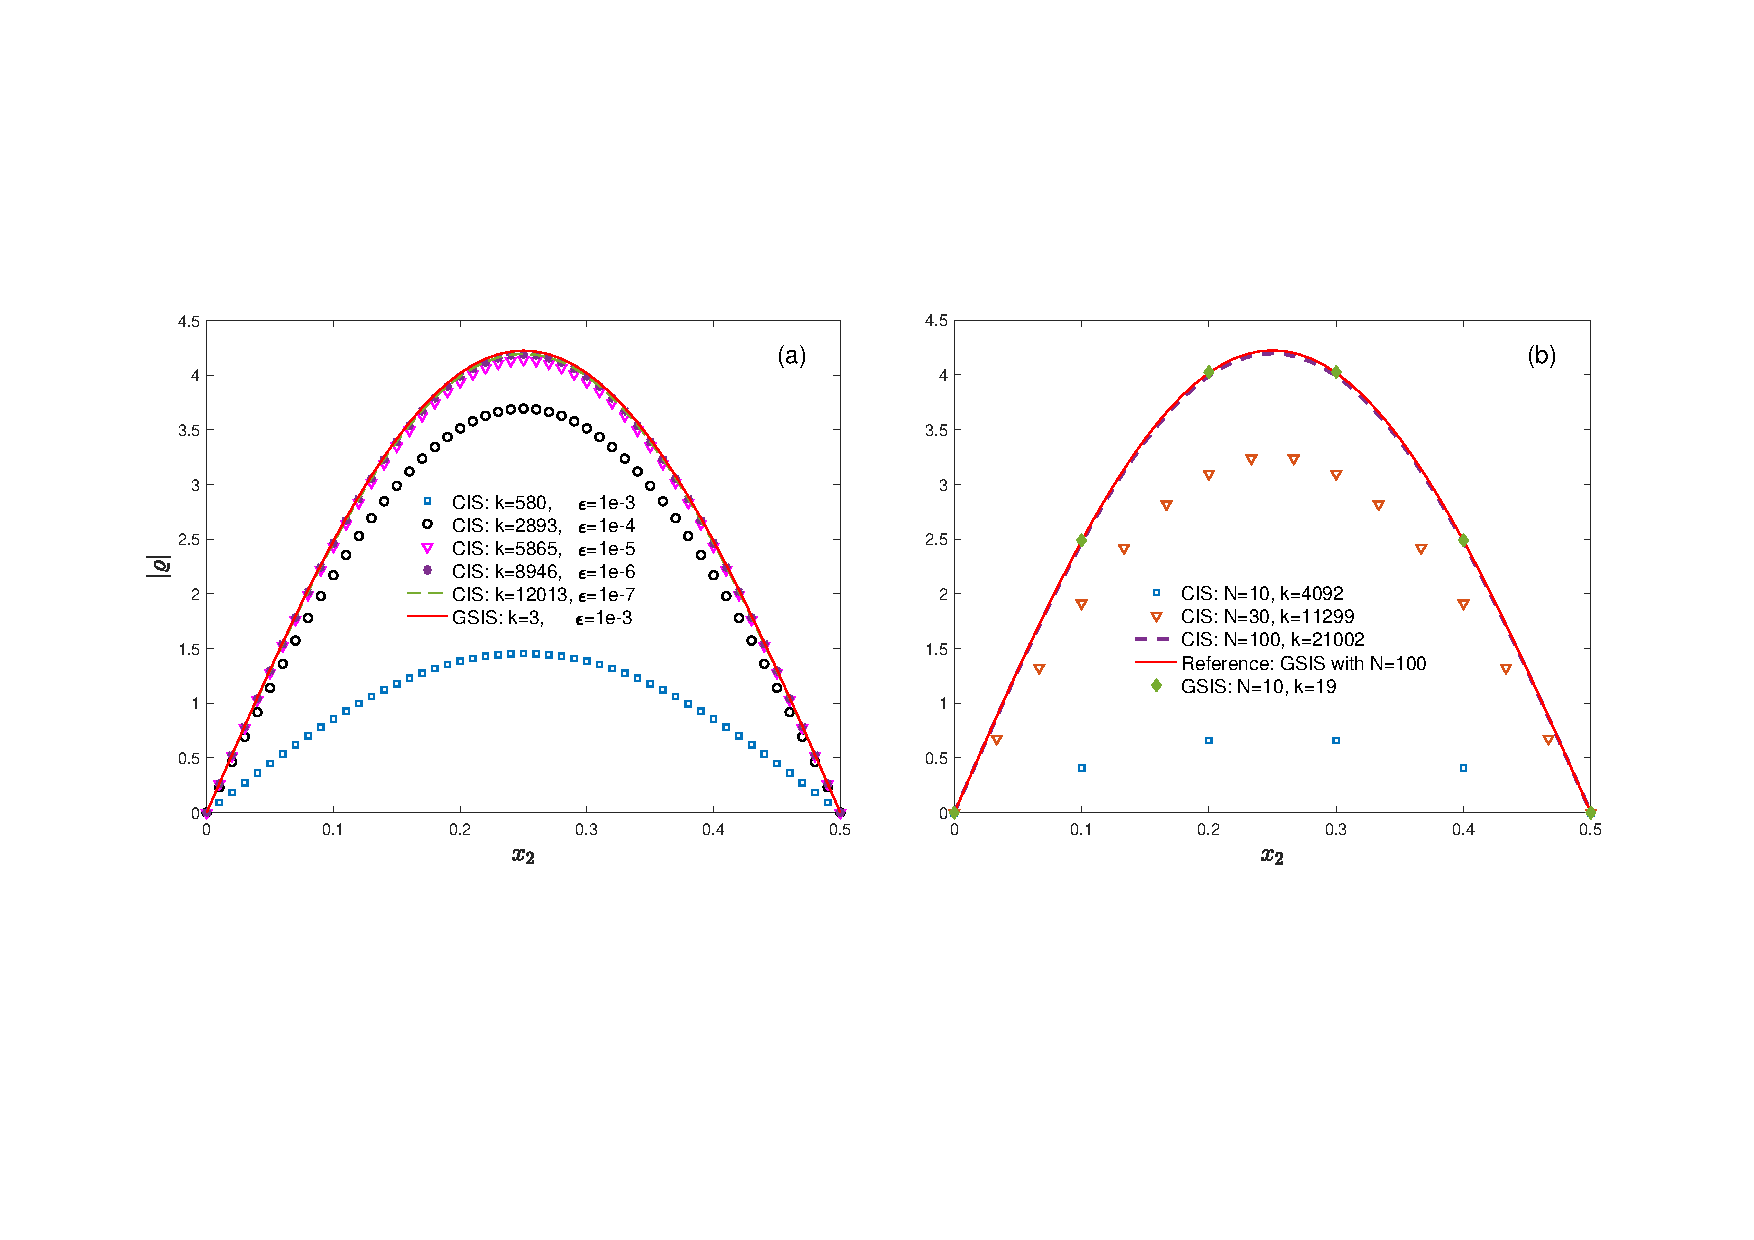
\includegraphics[width=1\columnwidth]{GSIS/IMG/Ke_5fs_resonant.pdf}
	\caption{Density profile in the coherent Rayleigh-Brillouin scattering~\cite{Su2020SIAM}, when $\delta_{rp}=200$. (a) The convergence history of CIS. The spatial region $x_2\in[0,1]$ is divided into $N=100$ uniform cells. Due to symmetry only half of the density profile is plotted.  (b) Density profiles and iteration numbers, where the iteration is terminated when $\epsilon<10^{-10}$. }
	\label{fig:CRBS_K_005}
\end{figure}

\begin{figure}[t]
	\centering
	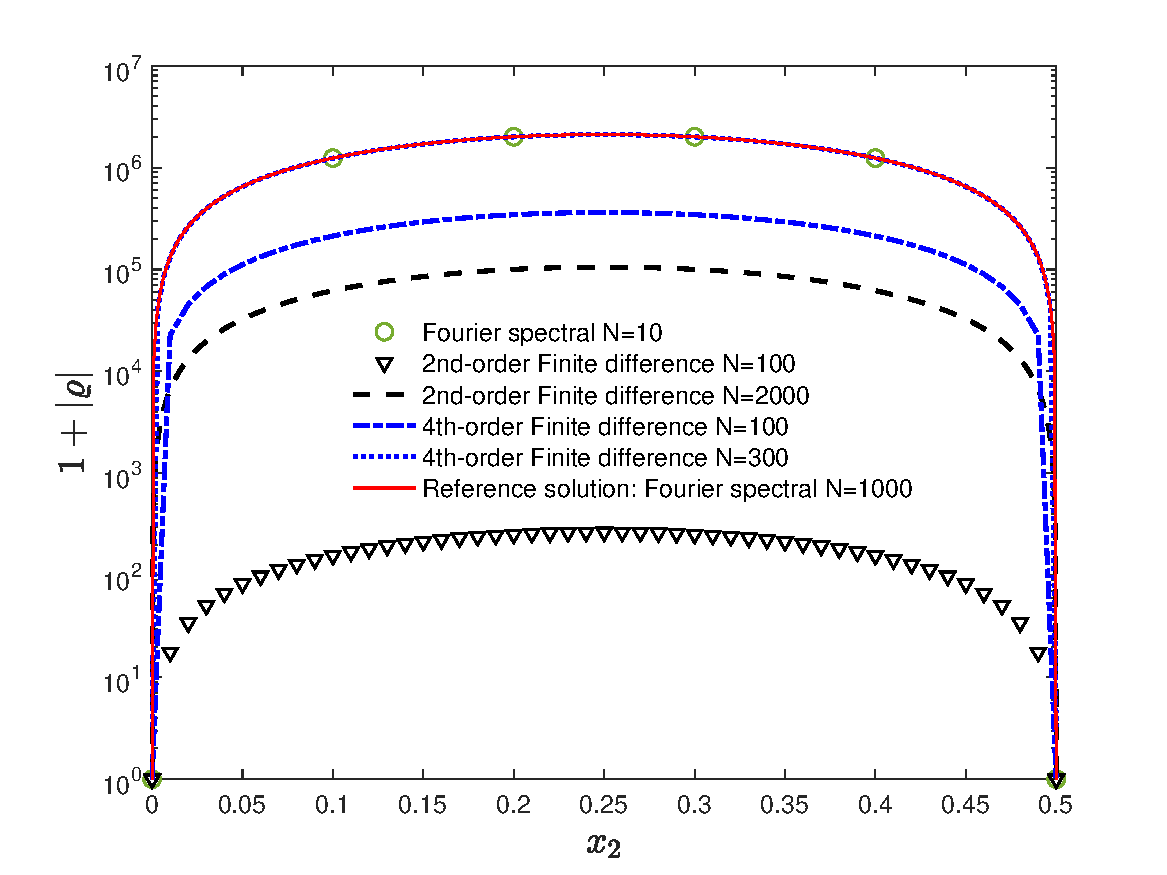
\includegraphics[width=0.7\columnwidth]{GSIS/IMG/crbsKn1e_8.pdf}
	\caption{Comparisons of the density profile in coherent Rayleigh-Brillouin scattering~\cite{Su2020SIAM}, where the kinetic equation is solved by the second-order upwind finite difference, while macroscopic equations are solved by various schemes with different number of spatial points ($N$). The Knudsen number is $K=10^{-8}$. The density amplitude is shifted by one in order to show it in the log scale. }
	\label{fig:crbsKn1e-8}
\end{figure}


We first consider the case where the kinetic and synthetic equations are solved by the second-order upwind finite difference and Fourier spectral methods, respectively. Figure~\ref{fig:CRBS_K_005}(a) shows the convergence history of both CIS and GSIS, when the rarefaction parameter is $\delta_{rp}=200$. It is clearly seen that, GSIS produces the converged solution after only 3 iterations, and when the convergence criterion 
\begin{equation}
\epsilon=\left|\frac{\int|\varrho^{(k+1)}dx_2|}{\int|\varrho^{(k)}|dx_2}-1\right|
\end{equation}
is $10^{-3}$. This is due to the super-converging property given in Eq.~\eqref{super_convergence}
However, due to the false convergence proven in Eq.~\eqref{false_convergence_CIS}, CIS needs huge number of iterations and the convergence criterion has to be set very small, i.e., $\epsilon=10^{-10}$ in this case. 


Figure~\ref{fig:CRBS_K_005}(b) shows that GSIS-I  asymptotically preserves the NSF limit, when only 10 uniform spatial cells are used. This is in agreement with the theoretical prove~\eqref{scaling1}. When the same number of spatial cells are used in CIS, the density amplitude is about 5 times smaller than the true solution, which indicates a strong numerical dissipation. Only when the number of cells is increased to 100 can the CIS capture the density profile at $\delta_{rp}=200$. Taking into account both the spatial discretization and iteration number, GSIS is about 6,000 times faster than CIS. 


We further consider an extreme case of $\delta_{rp}=10^{8}$. In this case, normally the Euler equation is used to describe the gas dynamics, and many kinetic schemes are proposed to asymptotically preserve the Euler limit. However, it should be emphasized that, Euler equation cannot be used here, otherwise the amplitude of perturbation will go to infinity due to the omission of viscosity. The extremely large value of $\delta_{rp}$ poses a grand challenge to the numerical method for kinetic equations, as any small value of numerical dissipation could easily contaminate the final solution, which leads to a significant smaller amplitude of density perturbation. Even at such a small Knudsen number, if the macroscopic equation is solved exactly (by the Fourier spectral method) and $\Delta{x}\sim{O(1)}$ is able to capture the spatial variation, GSIS has infinite order of accuracy, see the circles in Fig.~\ref{fig:crbsKn1e-8}. However, when the second-order finite difference scheme is used to solve the synthetic equations, we need more than 2000 spatial points to capture the density perturbation; this is understandable since the numerical dissipation (or numerical viscosity) $(\Delta{x})^2=2.5\times10^{-7}$ is larger than the physical viscosity (here it is reflected by the inverse rarefaction parameter). When the synthetic equations are solved by the fourth-order finite difference, we see that $N=100$ leads to wrong solutions, while $N=300$ yields accurate solution. This is because the numerical dissipation is about $(\Delta{x})^4=10^{-8}$ and $1.2\times10^{-10}$, respectively, so that the former is too dissipative while the latter is accurate.   

The last numerical example in Fig.~\ref{fig:crbsKn1e-8} illustrates the flexibility, importance, and advantage of GSIS that the kinetic and synthetic equations are solved by different methods with different order of accuracy. Since many sophisticated high-order methods have been developed for NSF equations, they can be directly incorporated in the GSIS framework to boost convergence and reduce the use of spatial cells and hence the computational memory.  


\subsection{Planar Fourier flow}
\index{Fourier flow}

We consider the heat conduction in gas between two plates located at $x_2=0$ and 1, see  Section~\ref{Fourier_lin_FSM}, the see the influence of solid walls in the fast-converging properties of GSIS. 

From the synthetic equations~\eqref{eq123}, \eqref{HoT_sigma} and~\eqref{HoT_q}, as well as the symmetry condition, we know $\bm{u}=0, \sigma_{ij}=0~ \text{when}~ i\neq{j}$, and $q_1, q_3=0$; the heat flux $q_2$ is a constant, and the perturbed temperature is governed by the following ordinary differential equation:
\begin{equation}\label{HoT_q_Fourier}
\begin{aligned}[b]
\frac{\partial T}{\partial x_2}=&-\frac{4\delta_{rp}}{9C_q}q_{2}+\underbrace{\frac{2}{3C_q}\int{}v_2v^2(\mathcal{L}-\mathcal{L}_{s})\mathrm{d}\bm{v}}_{H_1^{k}(x_2)}\\
&-\underbrace{\frac{2}{3C_q}\frac{\partial }{\partial x_2}\int{}(v_2^2-C_q)\left(v^2-\frac{3}{2}\right)h\mathrm{d}\bm{v}}_{H_2^{k+1/2}(x_2)},
\end{aligned}
\end{equation}
whose solution at the $(k+1)$-th iteration step is given by 
\begin{equation}
T^{k+1}(x_2)=-\frac{4\delta_{rp}{q}_2}{9C_q}\left(x_2-\frac{1}{2}\right)+\int_{1/2}^{x_2}H_1^{k}(x_2)\mathrm{d}x_2-H_2^{k+1/2}(x_2),
\end{equation}
where the constant heat flux $q_2$ is
\begin{equation}
q_2=\frac{9C_q}{2\delta_{rp}}\left[
T^{k+1/2}(0)+H_2^{k+1/2}(0)-H_1^{k}(0) \right].
\end{equation}


The density can be easily obtained by $\varrho+T+\sigma_{22}=0$, where from Eq.~\eqref{HoT_sigma} the stress $\sigma_{22}$ is calculated as
\begin{equation}\label{HoT_sigma_Fourier}
\sigma_{22} 
=-\frac{\frac{\partial}{\partial x_2}\int{}2v_{<2}v_{2>}v_2h\mathrm{d}\bm{v}}{\delta_{rp}}+\frac{2}{\delta_{rp}}\int{(\mathcal{L}-\mathcal{L}_s)v_2^2}\mathrm{d}\bm{v}.
\end{equation}


\begin{figure}[t]
	\centering
	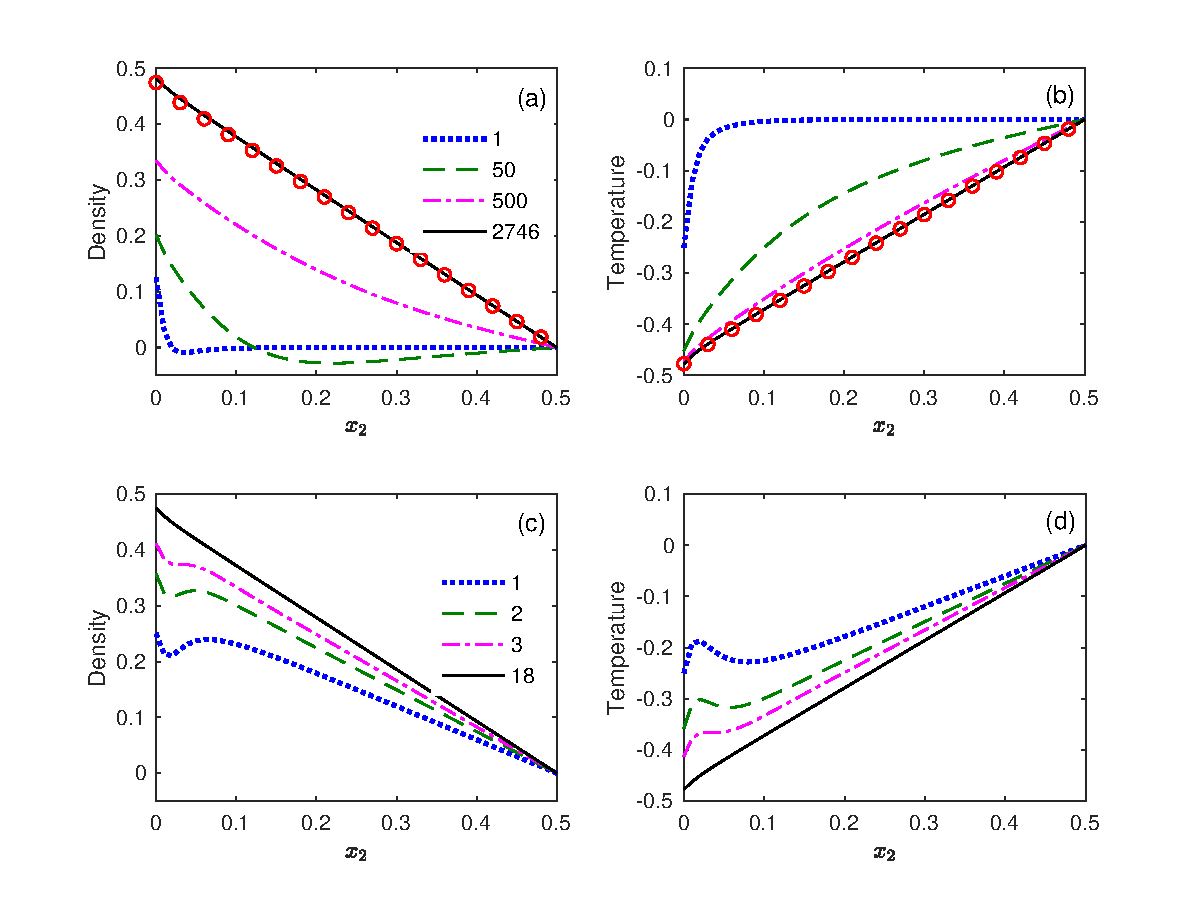
\includegraphics[scale=0.8,viewport=20 10 540 420,clip=true]{GSIS/IMG/Fourier_convergence_history.pdf}
	\caption{Convergence history in planar Fourier flow at $\delta_{rp} = 50$~\cite{SuArXiv2019}.  (Top) CIS, (Bottom) GSIS. Circles:  converged solution from GSIS. The linearized Shakhov model is used with the initial condition $h(x_2,\bm{v})=0$. Iteration steps are shown in the legends.}
	\label{fig:Fourier_histroy}
\end{figure}




%We choose the rarefaction parameter $\delta_{rp}=50$ and discretize the half spatial space into $N_2$ even-spaced points, where the derivative with respect to $x_2$ is approximated by a second-order upwind finite difference. The molecular velocity space in the $v_1$ and $v_3$ directions is truncated to the region $[-6, 6]$ by $24\times24$ equidistant points, while the molecular velocity $v_2$ is truncated to $[-6,6]$ and approximated by non-uniform points~\eqref{nonuniform_v}; in this test we take $\imath=3$ and $N_v=64$. Iterations in both CIS and GSIS are terminated when 
%\begin{equation}\label{epsilon_Fourier}
%\epsilon= \max\left\{
%\int{}\left|\frac{\varrho^{k+1}}{\varrho^{k}}-1\right|\mathrm{d}x_2, 
%\int{}\left|\frac{T^{k+1}}{T^{k}}-1\right|\mathrm{d}x_2,
%\int{}\left|\frac{q_2^{k+1}}{q_2^{k}}-1\right|\mathrm{d}x_2
%\right\}
%\end{equation}
%is less than a certain value. Note that  $\rho$ and $T$  at $x_2=1/2$ are excluded in the above equation since they are zero.


The efficiency of GSIS and CIS is compared in Fig.~\ref{fig:Fourier_histroy}. Starting from the initial condition $h(x_2,\bm{v})=0$, the perturbance from the solid surface quickly changes the density and temperature nearby in the CIS. However, the perturbance  can hardly penetrates into the bulk region. Such a slow convergence is completely changed in GSIS. As can be seen from Fig.~\ref{fig:Fourier_histroy}(d), after the first iteration, although the gas temperature near the wall is the same as that in CIS, the bulk temperature in GSIS is adjusted to be nearly linear, by the synthetic equation whose dominant parts are 
\begin{equation}
\frac{\partial T}{\partial x_2}=-\frac{4\text{Pr}\delta_{rp}}{5}q_{2}, \quad
\text{and} \quad
\varrho=-T.
\end{equation}
Then, due to the correction of VDF as per Eq.~\eqref{guided0}, at the second iterative step, the boundary condition~\eqref{Fourier_boundarycondition} in GSIS  is more close to the final steady-state than that in CIS. Hence after the second iteration, the GSIS results are closer to the final solution both at the boundary and in the bulk, i.e., fast convergence is achieved.	




\begin{figure}[t]
	\centering
	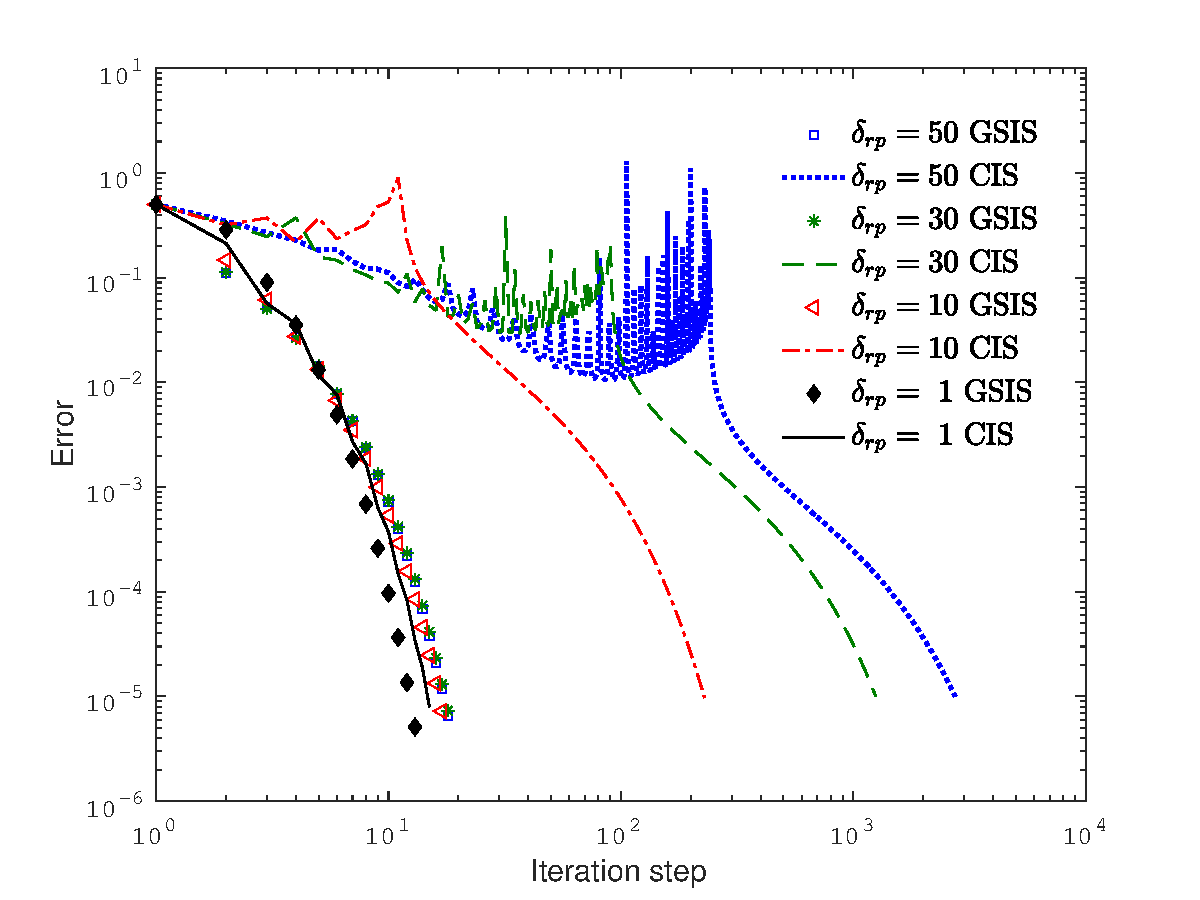
\includegraphics[width=0.7\columnwidth]{GSIS/IMG/Fourier_convergence_error.pdf}
	\caption{The decay of error $\epsilon$ as a function of the iteration step, for the Fourier flow between two parallel plates. The spatial region is discretized by 51 equidistant points.  }
	\label{fig:Fourier_speed}
\end{figure}

Figure~\ref{fig:Fourier_speed} shows the history of error decay of both CIS and GSIS, from the continuum  to transition flow regimes. In CIS, the number of iteration steps increases drastically with $\delta_{rp}$, while in GSIS converged solutions are found within 20 iterations for $\delta_{rp}=1$, 10, 30, and 50. Theoretically, according to Eq.~\eqref{super_convergence}, the number of iterations should be very small when $\delta_{rp}$ is large. This discrepancy is in fact caused by the present of solid wall, where the local Knudsen number inside the Knudsen layer is about 1, therefore, the effective error decay rate of GSIS, as shown in Fig.~\ref{fig:SR}, is about 0.5. This means that, for wall-bounded rarefied gas flows, the error is reduced by 3 orders of magnitude after 10 iterations in GSIS, no matter what the Knudsen number is. This explanation is in strong agreement with the results in Fig.~\ref{fig:Fourier_speed}. Therefore, in terms of fast-converging, GSIS-I and GSIS-II have similar performance. 




%Another important property of the GSIS is that the numerical error caused by the spatial discretization is much reduced when compared to that of CIS, thanks to the asymptotic preserving property of GSIS. From Fig.~\ref{fig:Fourier_spatial_error} we see that, in CIS, when the spatial cell size is 5 times of MFP, the relative error in density and heat flux are 9\% and 16\%, respectively. However, that in the GSIS always remain within 1\%. Even when $\delta_{rp}=500$, the heat flux obtained from the GSIS only changes from $3.721\times10^{-3}$ when $N_2=551$ to $3.726\times10^{-3}$ when $N_2=6$. The reason for this excellent performance is that the GSIS is asymptotically preserving the NSF limit, while in CIS the ``numerical'' thermal conductivity may be different to the physical one. 


%It should be noted that the implicit UGKS~\cite{zhuyajun2016} and other variants~\cite{yang2018PoF,yang2018PRE} can also produce accurate results when the cell size is much larger than the molecular MFP. This is achieved through a complex evaluation of the numerical flux at the cell interface to simultaneously handle the streaming and collision. GSIS, however, does not need complex flux evaluation since NSF constitutive laws are recovered explicitly. 




\subsection{Couette flow between eccentric cylinders}


Consider a Couette flow \index{Couette flow} between two non-coaxial cylinders in Fig.~\ref{TwoCylinderV}. The inner cylinder is stationary, while the outer cylinder rotates clockwise at a constant speed of $u_w$. The Shakhov model is linearized when $\beta$ in Eq.~\eqref{Chapter_lin_VDF} takes the value of $u_w/v_m$. The high-order discontinuous (DG) \index{discontinuous Galerkin} methods are employed to solve the linearized Shakhov model and synthetic equations, on structured triangular mesh~\cite{SuArXiv2019}.  



\begin{figure}[tp]
	\centering
	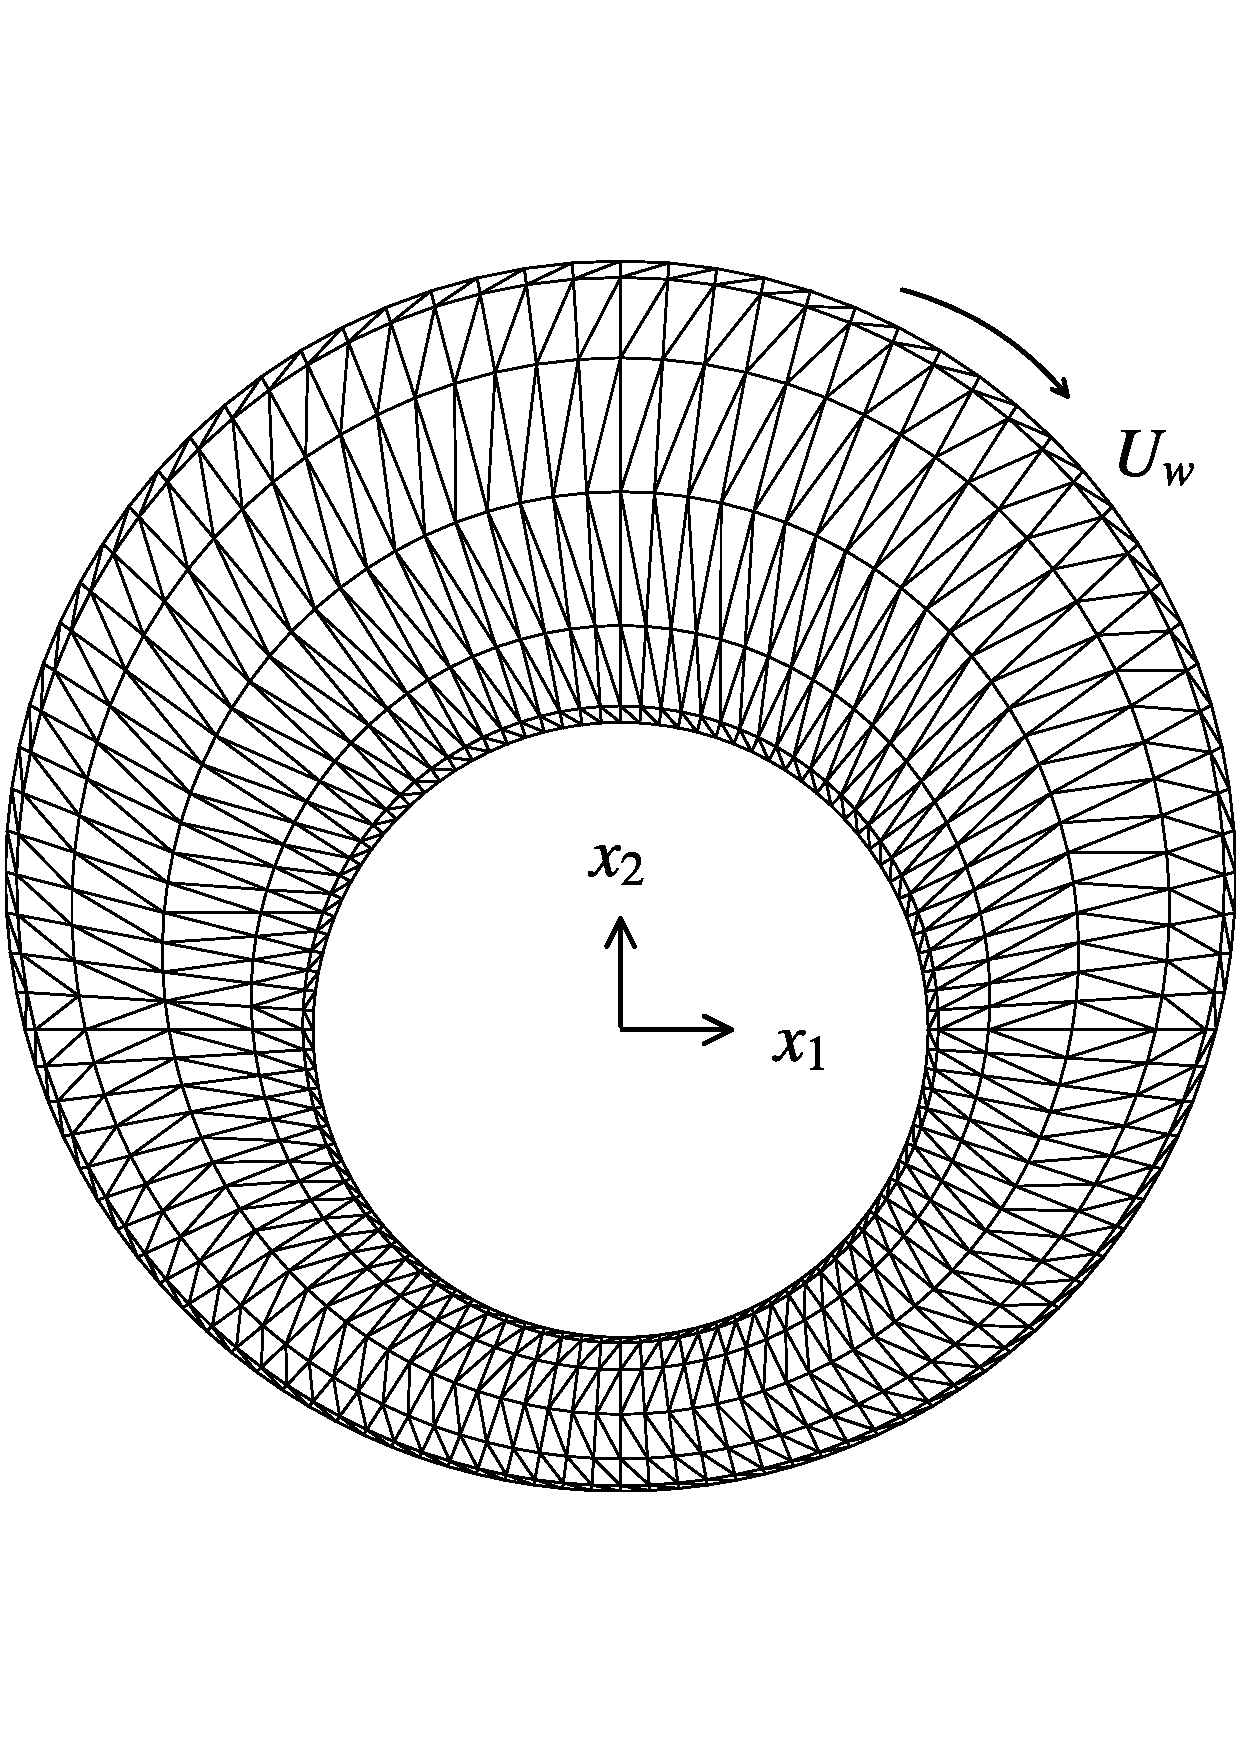
\includegraphics[width=0.3\textwidth]{GSIS/IMG/Cylinder_G.pdf}\\
	\vskip 0.5cm
	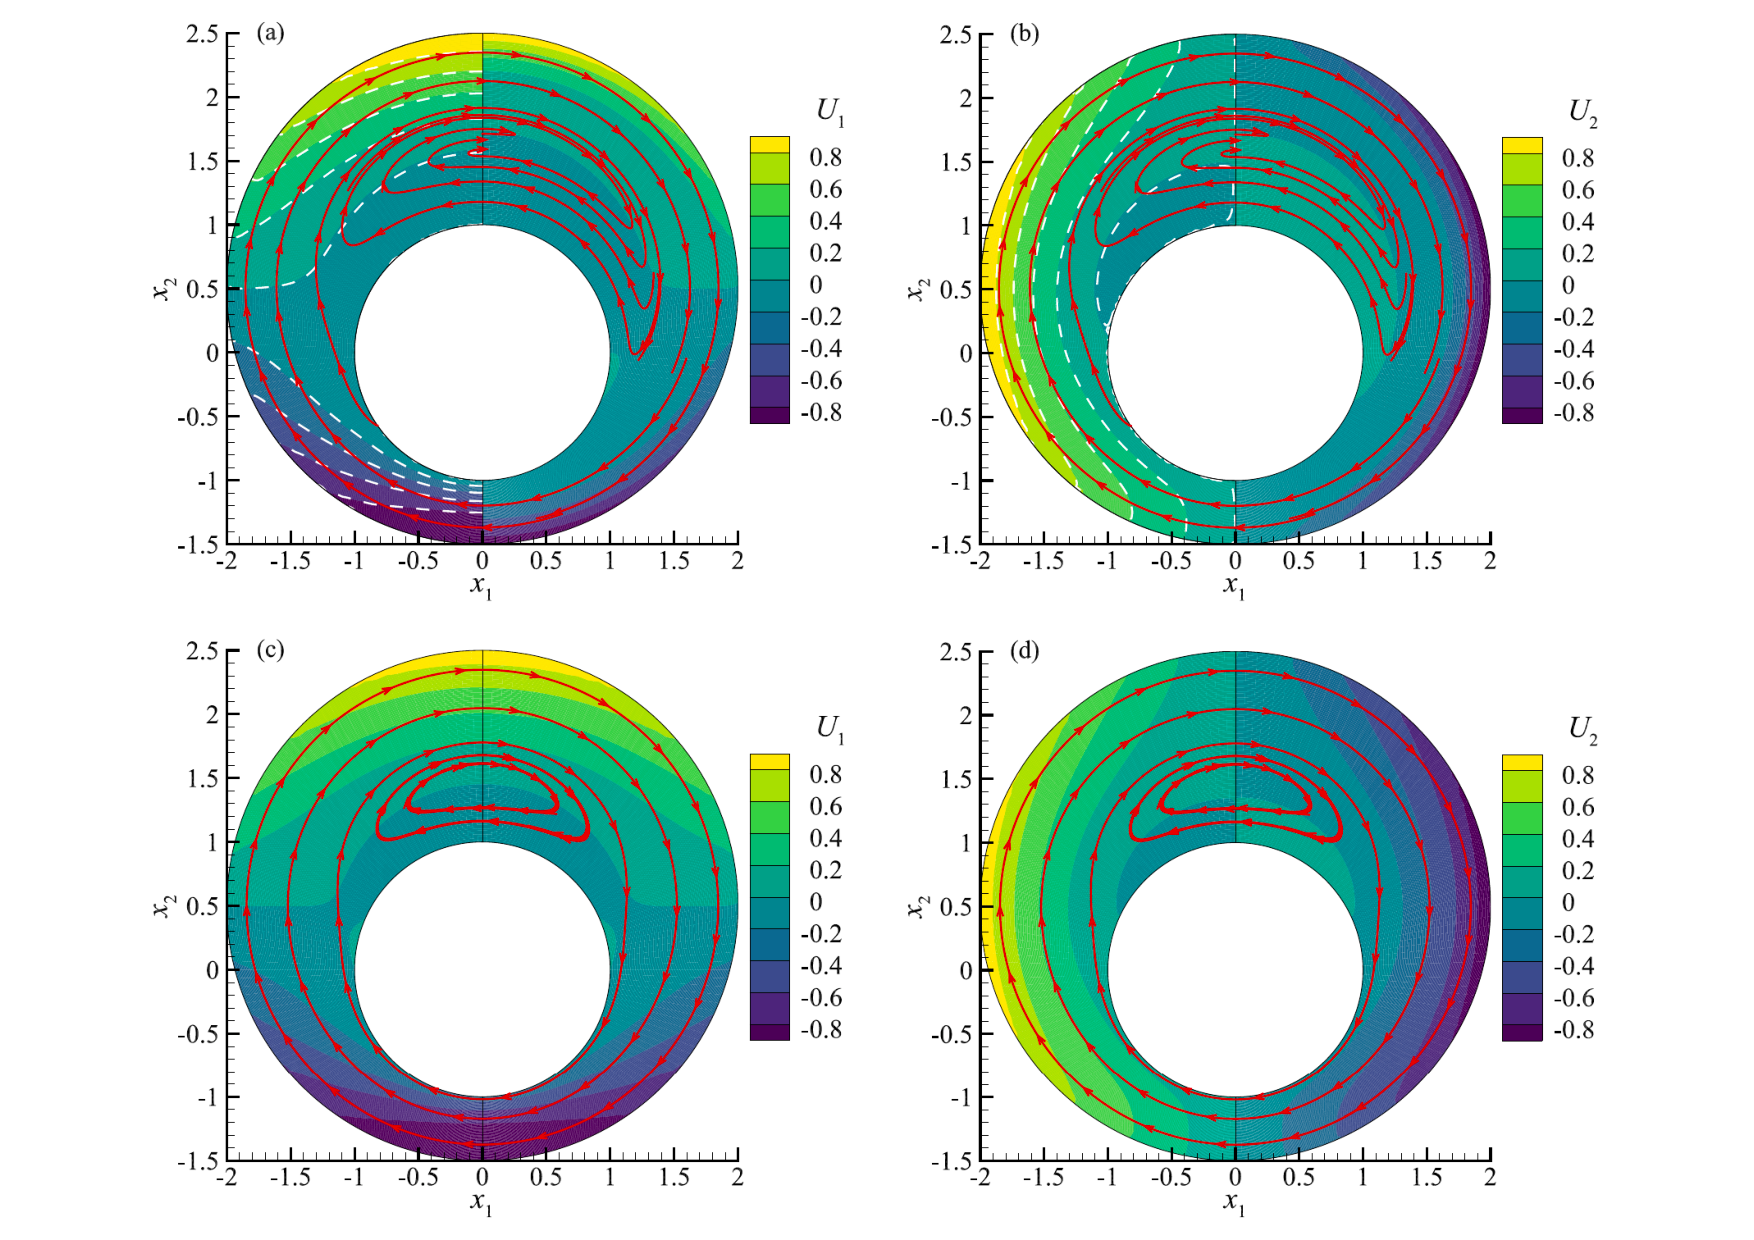
\includegraphics[width=0.9\textwidth]{GSIS/IMG/TwoCylinder.pdf}
	\caption{Contours and streamlines in the Couette flow between two eccentric cylinders~\cite{SuArXiv2019}. (a, b)  $\delta_{rp}=1000$. (c, d) $\delta_{rp}=10$. GSIS (CIS) results are plotted in the left (right) half domain. Dashed lines in (a) and (b):  velocity contours from the Navier-Stokes equations with non-slip velocity boundary.
	}
	\label{TwoCylinderV}
\end{figure}



Figure ~\ref{TwoCylinderV} shows the velocity contours and streamlines. When $\delta_{rp}=1000$, the flow is in the continuum regime, and the GSIS results overlap with the ones from the NSF equations even when the maximum cell size is about 260 times of MFP, which proves the asymptotically preserving property of GSIS.  However, the CIS fails to predict the velocity profile  due to its numerical dissipation on such a coarse mesh. When $\delta_{rp}=10$, CIS produces close solutions to GSIS,  because the mesh resolution is adequate. 

Table~\ref{tab:iteration2} shows the iteration numbers and CPU time. While GSIS obtains the converged solution within dozens of iterations, CIS needs 49454 and 296 iteration steps when $\delta_{rp}=1000$ and 10, respectively; as a result, GSIS is about 1300 and 5 times faster.



%. GSIS requires only 26 iterative steps to reach the convergence criterion for both cases, while CIS consumes  Compared to that of solving the kinetic equation, the computational consumption to solve the macroscopic equations is negligible. Therefore, 


\begin{table}[t]
	\centering
	\caption{Number of iteration steps and CPU time to reach convergence for the Couette flow between two eccentric cylinders~\cite{SuArXiv2019}. Iteration terminates when the relative error in flow velocity  between two consecutive iteration steps is less than $10^{-5}$. Simulations are run on 12 processors using OpenMP, on double precision Intel Xeon-E5-2680 processors. }
	\begin{tabular}{rllrrrr}
		\hline
		\multicolumn{1}{l}{$\delta_\text{rp}$} & Number of & Discrete    & \multicolumn{2}{c}{Iteration steps} & \multicolumn{2}{c}{CPU time (s)} \\ 
		&  triangles   &   velocities    & \multicolumn{1}{r}{CIS} & \multicolumn{1}{r}{GSIS} & \multicolumn{1}{r}{CIS} & \multicolumn{1}{r}{GSIS}\\ 
		\hline
		1000   & 2400 & $8\times8\times 12$ & 49454    & 26    &     33861.2  & 26.3 \\
		10  & 1600 & $32\times32\times 24 $& 296    & 26    &   2849.8    & 580.3 \\ 
		\hline
	\end{tabular}%
	\label{tab:iteration2}%
\end{table}


%\subsection{Thermal edge flow}\label{thermal_edge}
%\index{thermal edge flow}
%
%Consider a more challenging problem: a 2D flow induced by a hot beam that is encompassed in a cold chamber~\cite{Su2020SIAM}, see  Fig.~\ref{fig:Beam}(a). Both the beam and chamber are square, with dimensions of $2\times2$ and $8\times8$, respectively. The beam with a (deviated) temperature of $T=1$ is placed with distance of 1 away from the left and bottom walls of the enclosure. The chamber temperature is $T=0$ and a gas is filled between the beam and chamber. When the NSF equations are considered,  there is  no bulk flow, and the gas temperature is governed by Fourier's law of heat conduction. However, under the non-equilibrium circumstances, thermal stress and thermal edge flows are induced due to the rarefaction effects in Knudsen layer~\cite{Sone2002Book}. 
%
%\begin{figure}[h]
%	\centering
%	\includegraphics[trim=65 72 60 80, clip,scale=0.51]{GSIS/IMG/Beam} \includegraphics[trim=20 170 20 170,clip,scale=0.22]{GSIS/IMG/Beam_T}
%	\caption{Two-dimensional thermal flow induced by a square hot beam encompassed in a cold chamber when $\text{Kn}=0.001$. Schematic of (a) geometry and (b) spatial discretization of structured triangles with refinement in the vicinity of solid walls. (c) typical temperature contours obtained by DG schemes of $n_\text{K}=n_\text{S}=6$ and on spatial mesh of 16104 triangles~\cite{Su2020SIAM}. }
%	\label{fig:Beam}
%	%
%\end{figure}
%
%
%We calculate the thermal flow at a challenging Knudsen number of $\text{Kn}=0.001$, when the characteristic flow length is chosen as the gap between the beam and chamber. In addition to the fact that the flow viscosity of gas is small, the magnitude of bulk velocity is also small; in this case high resolutions of both Knudsen layer and bulk region are necessary, otherwise, under-resolution of the Knudsen layer and/or large numerical dissipation will introduce error at the same or even larger order  of the bulk velocity, which leads to completely wrong result. 
%
%
%The computational domain is partitioned by structured triangles with refinement in the vicinity of walls, see Fig.~\ref{fig:Beam}(b), which is characterized by the total number of triangles $N_\Delta$, the minimum cell size (the height of the local triangle) within Knudsen layer $L_\lambda$ and the maximum cell size in bulk region $L_\text{b}$. The diffuse BC is imposed on solid surfaces. The DG scheme \index{discontinuous Galerkin} is employed in the numerical simulation; the order of DG scheme for the kinetic equation is denoted by $n_\text{K}$, while that for synthetic equations is $n_\text{S}$.  Typical temperature field is shown in Fig.~\ref{fig:Beam}(c) that are obtained on the mesh of $N_\Delta=16104$, $\delta_{rp}L_\lambda=0.16$ and $\delta_{rp}L_\text{b}=128$ (i.e., the maximum cell size is 128 times of MFP) by the DG scheme with $n_\text{K}=n_\text{S}=6$. The BGK model is considered, and the molecular velocity space is discretized by $8\times8$-point Gauss-Hermite quadrature.
%
%
%
%
%
%\begin{figure}[t]
%	\centering
%	\includegraphics[trim=50 200 50 200, clip,scale=0.22]{GSIS/IMG/Beam_stream_a}\includegraphics[trim=50 200 50 200,clip,scale=0.22]{GSIS/IMG/Beam_stream_b}\includegraphics[trim=50 200 50 200,clip,scale=0.22]{GSIS/IMG/Beam_stream_c}\\
%	\includegraphics[trim=50 200 50 200,clip,scale=0.22]{GSIS/IMG/Beam_stream_d}\includegraphics[trim=50 200 50 200,clip,scale=0.22]{GSIS/IMG/Beam_stream_e}\includegraphics[trim=50 200 50 200,clip,scale=0.22]{GSIS/IMG/Beam_stream_f}
%	\caption{Streamlines obtained from DG schemes with different orders of accuracy and spatial meshes~\cite{Su2020SIAM}. (a) $\delta_{rp}L_\lambda=0.08$, $\delta_{rp}L_\text{b}=128$, and $n_\text{K}=n_\text{S}=2$;  (b) $\delta_{rp}L_\lambda=0.04$, $\delta_{rp}L_\text{b}=64$, and $n_\text{K}=n_\text{S}=2$; 
%		(c) $\delta_{rp}L_\lambda=0.32$, $\delta_{rp}L_\text{b}=256$, and $n_\text{K}=n_\text{S}=4$; 
%		(d) $\delta_{rp}L_\lambda=0.08$, $\delta_{rp}L_\text{b}=128$, and $n_\text{K}=n_\text{S}=6$; (e) $\delta_{rp}L_\lambda=0.08$, $\delta_{rp}L_\text{b}=128$, $n_\text{K}=2$ and $n_\text{S}=6$; (f) $\delta_{rp}L_\lambda=1.28$, $\delta_{rp}L_\text{b}=64$, and $n_\text{K}=n_\text{S}=4$.}
%	\label{fig:BeamStream}
%	%
%\end{figure}
%
%We first consider the flow pattern  in Fig.~\ref{fig:BeamStream}, which are obtained by the DG scheme of different orders and on different spatial meshes. On the same spatial mesh with cell size of 0.08 MFP in the Knudsen layer and 128 MFP in the bulk region, completely different flow patterns are obtained by second-order and sixth-order DG schemes, see Fig.~\ref{fig:BeamStream}(a) and (d). In the flow field predicted by the second-order scheme, four small vortices are generated around the lower-left corner of the beam; while another four are developed near the upper-right corner of the beam. At each of the lower-right and upper-left corners of the beam, three more vortices appear. Two small vortices are observed near the lower-right and upper-left corners of the chamber. On the other hand, from the sixth-order DG scheme, only eight vortices are developed, with each corner of the beam having two. Therefore, on this spatial grid ($\delta_{rp}L_\lambda=0.08$ and $\delta_{rp}L_\text{b}=128$), the second-order scheme produces larger errors; reducing the cell size by half is even not adequate, see Fig.~\ref{fig:BeamStream}(b). It is also worth noticing that only increasing the order of DG scheme for synthetic equations, the predicted flow field is still quiet different from that when the mesoscopic and macroscopic equations are all solved using sixth-order DG scheme, see flow field in Fig.~\ref{fig:BeamStream}(e) obtained on mesh of $\delta_{rp}L_\lambda=0.08$ and $\delta_{rp}L_\text{b}=128$ and schemes of $n_\text{K}=2$ and $n_\text{S}=6$. These results show the importance of resolving the Knudsen layer, where the non-equilibrium effects are the sources of gas motion. 
%
%\begin{figure}
%	\centering
%	\includegraphics[scale=0.4]{GSIS/IMG/Beam_Velocity}
%	\caption{Flow velocities obtained from DG schemes with different orders of accuracy and meshes with different cell sizes, in a two-dimensional thermal flow when $\delta_{rp}=1000$. (a) vertical velocity $u_2$ along the horizontal line at {$x_2=0.5$}; (b) vertical velocity $u_2$ along the horizontal at {$x_2=4.5$}. $\bar{L}_\lambda$ and $\bar{L}_\text{b}$ are the minimum cell size in Knudsen layer and maximum cell size in bulk region, respectively, which are normalized by the MFP of gas molecules, i.e., $\delta_{rp}\bar{L}_\lambda=L_\lambda$ and $\delta_{rp}\bar{L}_\text{b}=L_\text{b}$~\cite{Su2020SIAM}.}
%	\label{fig:BeamVelocity}
%\end{figure}
%
%To further demonstrate the importance of resolving the Knudsen layer, we use the fourth-order DG scheme to solve the kinetic and synthetic equations on two different meshes: Fig.~\ref{fig:BeamStream}(c) is obtained when  $\delta_{rp}L_\lambda=0.32$ and $\delta_{rp}L_\text{b}=256$, while Fig.~\ref{fig:BeamStream}(f) is obtained when $\delta_{rp}L_\lambda=1.28$ and $\delta_{rp}L_\text{b}=64$. Figure~\ref{fig:BeamStream}(c) shows that, on the mesh where the Knudsen layer is resolved by relatively fine cells, the flow pattern with eight vortices are developed, which are very similar to the high resolution results in Fig.~\ref{fig:BeamStream}(d), despite that the cell size in the bulk region is relatively large. However, when the bulk region is partitioned by fine cells but the Knudsen layer is under resolved by coarse cells, Figure~\ref{fig:BeamStream}(f) shows that although eight vortices can be observed, large errors appear near the walls, where gas seems to penetrate the solid walls.
%
%
%
%
%
%
%\begin{table}[t]
%	\caption{The number of iterative steps (Itr), the mean velocity magnitude $|\bar{\bm{u}}|_{x_1=0.5}$ along the horizontal line $x_2=0.5)$, as well as the computational time $t_\text{c}$ under different combinations of spatial meshes and schemes, in a 2D thermal flow with $\delta_{rp}=1000$~\cite{Su2020SIAM}. $N_\Delta$ is the number of triangles in a mesh, $L_{\lambda}$ is the minimum cell size (triangle height) in Knudsen layer and $L_\text{b}$ is the maximum cell size in bulk region. `Err' is the relative error of the mean velocity magnitude $|\bar{\bm{u}}|$ compared to the reference one obtained with $N_\Delta=20424$, $\delta_{rp}L_{\lambda}=0.08$, $\delta_{rp}L_\text{b}=128$ and $n_\text{K}=n_\text{S}=6$. The computational time $t_\text{c}$ is the wall time cost by each case that runs on 8 Intel Xeon-E5-2680 CPUs using OpenMP. } % 
%	\centering
%	\begin{tabular}{ccccccccc}
%		\hline
%		$N_{\Delta}$ & $\delta_{rp}{L_{\lambda}}$ & $\delta_{rp}{L_{b}}$ & $n_\text{K}$ & $n_\text{S}$ & $|\bar{\bm u}|\times10^6$ &  Err [\%] & Itr & $t_\text{c}$ [h] \\
%		\hline
%		8832  & 0.32 & 256 & 4 & 4 & 1.072 & 7.4 & 49 & 0.01\\
%		16104 & 0.16 & 128 & 4 & 4 & 1.060 & 6.2 & 46 & 0.02\\
%		24864 & 1.28 & 64  & 4 & 4 & 1.077 & 7.9 & 45 & 0.06\\
%		30176 & 0.32 & 64  & 4 & 4 & 1.013 & 1.5 & 48 & 0.04 \\
%		33024 & 0.16 & 64  & 4 & 4 & 1.013 & 1.5 & 46 & 0.04 \\
%		8832  & 0.32 & 256 & 6 & 6 & 0.982 & 1.6 & 57 & 0.07 \\
%		10400 & 0.16 & 256 & 6 & 6 & 0.991 & 0.7 & 55 & 0.12 \\
%		16104 & 0.16 & 128 & 6 & 6 & 0.991 & 0.7 & 54 & 0.18 \\
%		20424 & 0.08 & 128 & 6 & 6 & 0.998 & 0 & 60 & 0.21 \\
%		\hline
%	\end{tabular}
%	\label{Tab:Beam}
%\end{table}
%
%
%To quantitatively show the accuracy and efficiency of numerical simulations, we plot the vertical velocity along the horizontal lines $x_2=0.5$ and $x_2=4.5$ in Fig.~\ref{fig:BeamVelocity}. As the refinement of spatial mesh and increment of the order of DG scheme, the flow properties converge to the reference ones (red solid lines) obtained on the mesh of $\delta_{rp}L_\lambda=0.08$ and $\delta_{rp}L_\text{b}=128$ and by sixth-order DG scheme. 
%In Table~\ref{Tab:Beam} we list the mean velocity along the horizontal line:
%\begin{equation}
%|\bar{\bm{u}}|=\frac{1}{8}\int^8_0|\bm{u}|(x_1,x_2=0.5)dx_1.
%\end{equation}
%The relative error between the mean velocity from the mesh of $\delta_{rp}L_\lambda=0.08$ and $\delta_{rp}L_\text{b}=128$ by sixth-order DG scheme and the one from the mesh of $\delta_{rp}L_\lambda=0.16$ and $\delta_{rp}L_\text{b}=256$ by the same order schemes is within 1\%, which indicates the accuracy of the reference result. The results for $|\bar{\bm{u}}|$ with different spatial discretizations and different orders of DG schemes clearly demonstrate the importance of resolving the Knudsen layer. 
%
%The iteration steps and computational time cost by each case are also listed in Table~\ref{Tab:Beam}. For all the cases, GSIS can find the steady-state solution with 50 to 60 steps. The computational time to obtain accurate solution (with less than 2\% error in $|\bar{\bm{u}}|$ compared to the reference one) can be as little as several minutes. To the best of our knowledge, we find no other numerical methods that are able to obtain accurate results within such a short time~\cite{Torrilhon2021_Compare,XU_AIA_compare}.   
%
%%We plotted the error $\epsilon$ as a function of the iteration step in Fig.~\ref{fig:BeamRes} for selected spatial meshes and DG resolutions. The presence of the sharp corners of the beam and chamber leads to strong variations (probably unphysical ones) in the macroscopic quantities at the beginning of the iteration. Therefore, during the first 20 iteration steps, the error decreases slowly and even goes up at some iteration steps. After that, however, the error declines continuously and rapidly, i.e., by 2 orders of magnitude within 10 iterations. 
%
%
%
%
%
%%\begin{figure}[t]
%%	\centering
%%	\includegraphics[scale=0.45]{Beam_Residual}
%%	\caption{The error decay history in the two-dimensional thermal edge flow with $\text{Kn}=0.001$. }
%%	\label{fig:BeamRes}
%%	% The relaxation coefficient is dependent on the local Knudsen number, according to Eq.~\eqref{Kn_loc}. The maximum cell size in the bulk region is $L_\text{b}/K=128$, which results in the minimum local Knudsen number about 0.008. The maximum local Knudsen number for the meshes of $L_\lambda/K=0.16$ and 0.08 is 6.8 and 14.4, respectively.
%%\end{figure}
%
%
%
%%
%%\section{Molecular gas}
%%
%%Wei's CMAME paper
%%\newpage
%%a
%%\newpage
%%b
%%\newpage
%
%
%
%
%%\section{Time-dependent problems}
%%
%%
%%%\subsection{Conventional iterative scheme}
%%
%%\index{Conventional iterative scheme}
%%
%%A direct method to solve the kinetic equation, which is a complicated integro-differential equation, is the use of  conventional iteration scheme. In this paper, we consider the following typical temporal discretization  for unsteady problems: 
%%\begin{equation}\label{Shakhov_time_dependent0}
%%\frac{h_{n+1}-h_n}{\Delta{t}}+
%%\frac{\bm{v}}{2}\cdot
%%\left( \frac{\partial{h_{n+1}}}{\partial\bm{x}}
%%+ \frac{\partial{h_{n}}}{\partial\bm{x}}\right) =r\mathcal{L}_{n+1}+(1-r)\mathcal{L}_{n}, 
%%\end{equation}
%%where the quantities with the subscript $n$ are evaluated at the time $t_n$, $\Delta{t}=t_{n+1}-t_{n}$ is the time step, and the parameter $r$ varies between 0.5 and 1~\cite{Taitano2014,Zhu2019JCP}. When $r=1/2$, the scheme is second-order accuracy in time, while when $r=1$ it is a backward Euler scheme with first-order temporal accuracy.
%%
%%
%%Since $\mathcal{L}_{n+1}$ is a function of $h_{n+1}$, Eq.~\eqref{Shakhov_time_dependent0} must be solved iteratively. In CIS, given the value of velocity distribution function $h_{n+1}^{k}$ at the $k$-th iteration step (this is often called inner iteration in time-dependent implicit schemes~\cite{Zhu2019JCP}), its value at the next iteration step is calculated by:
%%\begin{equation}\label{Shakhov_time_dependent}
%%\frac{h^{k+1}_{n+1}-h_n}{\Delta{t}}+
%%\frac{\bm{v} }{2}\cdot
%%\left( \frac{\partial{h^{k+1}_{n+1}}}{\partial\bm{x}}
%%+ \frac{\partial{h_{n}}}{\partial\bm{x}}\right) =r\left({\mathcal{L}_{n+1}^{+,k}- \delta_{rp}  h_{n+1}^{k+1}}\right)
%%+(1-r){ \mathcal{L}_{n} },
%%\end{equation}
%%and this process repeats until the relative difference in macroscopic quantities between two consecutive inner iterations are less than a fixed value. 
%%
%%
%%
%%
%%
%%
%%
%%\begin{figure}[t]
%%	\centering
%%	\includegraphics[scale=0.5]{omega_time_dependent.pdf}\\
%%	\includegraphics[scale=0.5]{omega_time_dependent_theta10.pdf}
%%	\caption{
%%		The error decay rate as a function of the  Knudsen number in CIS, GSIS, and HOLO~\cite{Taitano2014}, when $r=1/2$. Note that the iteration is unstable when the error decay rate is larger than one. 
%%	}
%%	\label{fig:GSIS12_time_dependent}
%%\end{figure}
%%
%
%
%





%The error decay rate for both the BGK and Shakhov models are shown in Fig.~\ref{fig:GSIS12_time_dependent}. It is clear that when the Knudsen number  is large, $e$ goes to zero so that the error decays quickly. This means that CIS is very efficient for highly rarefied gas flows, i.e., the converged solution can be found within dozens of iterations~\cite{SuArXiv2019}. On the contrary, $e\rightarrow1$ when $\text{Kn}\rightarrow0$, which means that the CIS is extremely slow in the (near) continuum flow regime. 
%
%
%%Specifically, when $\text{Kn}\rightarrow0$, we find in that the error decay rate can be calculated analytically as:
%%\begin{equation}\label{analytical_CIS}
%%e_{CIS}=1-\frac{1}{2\delta^2_{rp}}. \leir{\text{~~should be related to~} |\theta|}
%%\end{equation}
%
%
%
%
%
%\subsection{Scheme-II GSIS}\label{section_GSIS2}
%
%To expedite the convergence of inner iteration, that is, to reduce the number of $k$ in Eq.~\eqref{Shakhov_time_dependent}, synthetic equations are needed. There are several ways of constructing these equations, and we first develop the GSIS-II for time-dependent problems due to its relative simplicity~\cite{Zhu2021JCP}. 
%
%First, in GSIS, given the value of velocity distribution function $h_{n+1}^{k}$ at the $k$-th iteration step, its value at the intermediate $(k+1/2)$-th step is obtained in a similar way to Eq.~\eqref{Shakhov_time_dependent}:
%\begin{equation}\label{Shakhov_time_dependent_intermediate}
%\frac{h^{k+1/2}_{n+1}-h_n}{\Delta{t}}+
%\frac{\bm{v} }{2}\cdot
%\left( \frac{\partial{h^{k+1/2}_{n+1}}}{\partial\bm{x}}
%+ \frac{\partial{h_{n}}}{\partial\bm{x}}\right) =r\left({\mathcal{L}_{n+1}^{+,k}- \delta_{rp}  h_{n+1}^{k+1/2}}\right)
%+(1-r){ \mathcal{L}_{n} }. 
%\end{equation}
%This velocity distribution function $h^{k+1/2}_{n+1}$ will be used to construct high-order constitutive relations in synthetic equations; and when the synthetic equations are solved to obtain macroscopic quantities, say, $M^{k+1}_{n+1}=[\varrho,\bm{u}, T,\bm{q}]$,  they will be used in the gain term~\eqref{LBE_Shakhov} for the next inner iteration, until convergence criterion is met. % the velocity distribution function will be updated, and
%
%
%Certainly, the synthetic equations should be derived exactly from the gas kinetic model. In GSIS-II, the constitutive relations are constructed, with a free parameter $\delta$, in the following manner~\cite{Zhu2021JCP}:
%\begin{eqnarray}
%\sigma^{k+1}_{ij} =-2\delta^{-1}\frac{\partial u^{k+1}_{<i}}{\partial {x_{j>}}}
%+\left(\sigma^{k+1/2}_{ij} +2\delta^{-1}\frac{\partial u^{k+1/2}_{<i}}{\partial {x_{j>}}}\right), \label{sigma_HoT}\\
%q^{k+1}_i =-\frac{5}{4\mathrm{Pr}}\delta^{-1} \frac{\partial T^{k+1}}{\partial x_i}+
%\left(q_i^{k+1/2} +\frac{5}{4\mathrm{Pr}}\delta^{-1} \frac{\partial T^{k+1/2}}{\partial x_i}\right). \label{q_HoT}
%\end{eqnarray}
%
%
%

%
%
%%In GSIS, the velocity distribution function $h^{k+1}_{n+1}$ in Eq.~\eqref{Shakhov_time_dependent} is replaced by $h^{k+1/2}_{n+1}$, and after obtaining  $h^{k+1/2}_{n+1}$ the macroscopic quantities which will be used in the next inner iteration is calculated as (again, the Crank-Nicolson scheme is used)
%
%The synthetic equations are solved by the following Crank-Nicolson scheme (although other schemes can also be used):
%\begin{equation}\label{eq123_lin_time_dependent}
%\begin{aligned}[c]
%\frac{\varrho^{k+1}}{\Delta{t}}
%+\frac{1}{2}\frac{\partial {u^{k+1}_i}}{\partial{x_i}}=&\frac{\varrho_n}{\Delta{}t_n}
%-\frac{1}{2}\frac{\partial {u_{i,n}}}{\partial{x_i}},\\
%2\frac{u_i^{k+1}}{\Delta{t}}
%+\frac{1}{2}\frac{\partial }{\partial{x_i}}
%\left(
%\varrho^{k+1}+ {T^{k+1}}+\sigma^{k+1}_{ij}\right)
%=&
%2\frac{u_{i,n}}{\Delta{t}}
%-\frac{1}{2}\frac{\partial }{\partial{x_i}}\left(
%{\varrho_n}+T_n+\sigma_{ij,n}\right), \\
%\frac{3}{2}\frac{T^{k+1}}{\Delta{t}}
%+\frac{1}{2}\frac{\partial {{q^{k+1}_{i}}}}{\partial{x_i}}
%+\frac{1}{2}\frac{\partial {{u^{k+1}_{i}}}}{\partial{x_i}}=
%&\frac{3}{2}\frac{T_n}{\Delta{t}}
%-\frac{1}{2}\frac{\partial {q_{i,n}}}{\partial{x_i}}
%-\frac{1}{2}\frac{\partial {u_{i,n}}}{\partial{x_i}},	
%\end{aligned}
%\end{equation}
%where terms in the left-hand-side are evaluated at the $(n+1)$-th time step (for clarity the subscript is ignored), while these on the right-hand-side are evaluated at the $n$-th time step.
%
%
%
%%\subsubsection{Scheme II}
%
%
%
%A comparison of GSIS-II and HOLO is shown in Fig.~\ref{fig:GSIS12_time_dependent}, which clearly show that HOLO is unstable at large time step, say, when $\Delta{t}=15$ and $|\bm{\theta}|=1$. When the perturbation wavevector $\theta$ is increased, the time step for stable iteration in HOLO is much reduced, while the GSIS is always stable, see the last subfigure. 
%%\footnote{In fact, in the GSIS for steady-state solution of Boltzmann equation and kinetic model equations, we have chosen $\Delta{t}=\infty$ and we have shown that the GSIS is stable, both analytically and numerically~\cite{Su2020SIAM}.}; 
%
%
%%\vskip 3cm
%%\lei{write the detailed form of $L_8$ and $R_8$, please}
%%
%%\vskip 3cm

%% ----------------- do not delete -----------------

%\leir{
%However, the error decay rate increases to one when $\text{Kn}\rightarrow\infty$. To fix this problem, macroscopic quantities at the (k+1)-th iteration step are not all updated by the solution $M_{\text{syn}}$ from synthetic equations, when the Knudsen number is large. Rather, they are updated in the following manner
%\begin{equation}\label{GSIS_K3}
%M^{k+1}(\bm{x}\,)=\beta{}M_{\text{syn}}(\bm{x})+(1-\beta)M^{k+1/2}(\bm{x}),
%\end{equation}
%where the relaxation parameter $\beta$ is chosen as
%\begin{equation}\label{relax_parameter}
%\beta=\frac{\delta_{rp}}{\text{max}(\delta_{rp},\delta_{rp}^\text{th})}.
%\end{equation}
%with $\delta_{rp}^\text{th}$ being the threshold rarefaction parameter. That is, $\beta=1$ when the rarefaction parameter is larger than $\delta_{rp}^\text{th}$; when $\delta_{rp}<\delta_{rp}^\text{th}$, $\beta$ gradually decreases to zero as the Knudsen number approaches infinity. The error decay rate of GSIS can be obtained by computing the eigenvalue of the matrix
%\begin{equation}
%G=\beta{L_8^{-1}R_8}+(1-\beta)C_8,
%\end{equation} 
%where the results at different values of $\delta_{rp}^\text{th}$ are shown in Fig.~\ref{fig:SR}. Clearly, by choosing approximate value of $\beta$, we can make the maximum error decay rate less than 0.5 for all Knudsen number; this means that the error can be reduced by at least three orders of magnitude in 10 iterations. Thus, theoretically, GSIS can reach fast convergence in the whole range of Knudsen number.
%}









%\subsection{Scheme-I GSIS}\label{section_GSIS1}
%
%This time-dependent scheme is modified from  Ref.~\cite{SuArXiv2019} which is initially developed to find steady-state solutions of the Boltzmann equation and kinetic model equations. In addition the the five macroscopic equations from the mass, momentum and energy consecration~\eqref{eq123}, evolution equations for the stress and heat flux are also included, like that in the Grad 13 moment equations~\cite{Grad1949}. That is,  we multiply Eq.~\eqref{bgkfd} by $v_{\langle{i}}v_{j\rangle}$ and integrate the resultant equation with respect to the molecular velocity $\bm{v}$, and obtain 
%\begin{equation}\label{HoT_sigma0_TD}
%\frac{\partial \sigma_{ij}}{\partial {t}}
%+2\int{v_{\langle{i}}v_{j\rangle}} \bm{v}\cdot\frac{\partial h}{\partial \bm{x}}d\bm{v}=-\delta_{rp}\sigma_{ij}.
%\end{equation}
%However, unlike the Grad 13 moment system where the high order term (i.e. the second term in the left-hand-side) is closed by expanding the velocity distribution function into Hermite polynomial of molecular velocity, in GSIS-I Eq.~\eqref{HoT_sigma0_TD} is rearranged in the following form to reflect Newton's law for shear viscosity, which shall allow numerical stability at large time steps:
%\begin{equation}\label{HoT_sigma_TD}
%\begin{aligned}[c]
%\frac{\partial \sigma_{ij}}{\partial {t}}
%&+\underbrace{2\int{v_{\langle{i}}v_{j\rangle}} \bm{v}\cdot\frac{\partial h}{\partial \bm{x}}d\bm{v}-2\frac{\partial{u_{<i}}}{\partial {x_{j>}}}}_{\text{HoT}_{\sigma_{ij}}}
%+\underbrace{2\frac{\partial{u_{<i}}}{\partial {x_{j>}}}=-\delta_{rp}\sigma_{ij}}_{\text{Newton's law}}.
%\end{aligned}
%\end{equation}
%This equation is solved, again, by the Crank-Nicolson scheme:
%\begin{equation}\label{HoT_sigma2}
%\begin{aligned}[c]
%\left(\frac{1}{\Delta{t}}
%+\frac{\delta_{rp}}{2}\right)
%&\sigma^{k+1}_{ij}
%+\frac{\partial{u^{k+1}_{<i}}}{\partial {x_{j>}}}
%\\
%&=\left[\left(\frac{1}{\Delta{t}}-\frac{\delta_{rp}}{2}\right)\sigma_{ij,n}
%-\frac{\partial{u_{<i,n}}}{\partial {x_{j>}}}-\frac{\text{HoT}_{\sigma_{ij},n}}{2}
%\right]
%-\frac{\text{HoT}^{k+1/2}_{\sigma_{ij}}}{2}.
%\end{aligned}
%\end{equation}
%It is noted that, when the inner iteration converges,  $\text{HoT}^{k+1/2}_{\sigma_{ij}}$ will be the same as $\text{HoT}^{k+1}_{\sigma_{ij}}$, and hence this numerical scheme is a Crank-Nicolson scheme with second-order accuracy in time.
%
%
%Likewise, we multiply Eq.~\eqref{bgkfd} by $v_i(v^2-5/2)$ and integrate the resultant equation with respect to $\bm{v}$; we obtain 
%\begin{equation}\label{HoT_q_TD}
%\begin{aligned}
%\frac{\partial q_{i}}{\partial {t}}
%&+\underbrace{ \int{\left(v^2-\frac{5}{2}\right)}v_i \bm{v}\cdot\frac{\partial h}{\partial \bm{x}}d\bm{v}
%	-\frac{5}{4}\frac{\partial{T}}{\partial {x_{i}}
%} }_{\text{HoT}_{q_i}} 
%+\underbrace{\frac{5}{4}\frac{\partial{T}}{\partial {x_{i}}}=-\delta_{rp}\text{Pr}q_{i}}_{\text{ Fourier's law}},
%\end{aligned}
%\end{equation}
%which can also be solved by the Crank-Nicolson scheme.
%
%% as
%%\begin{equation}
%%\begin{aligned}[c]
%%\left(\frac{1}{\Delta{t}}+\frac{\delta_{rp}}{2}\text{Pr}\right)
%%&q^{k+1}_{i}
%%+\frac{5}{8}\frac{\partial T^{k+1}}{\partial x_i}
%%\\
%%&=\left[\left(\frac{1}{\Delta{t}}-\frac{\delta_{rp}}{2}\text{Pr}\right)q_{i,n}
%%-\frac{5}{8}\frac{\partialT_n}{\partial x_i}-\frac{\text{HoT}_{q_{i},n}}{2}
%%\right]
%%-\frac{\text{HoT}^{k+1/2}_{q_{i}}}{2}.
%%\end{aligned}
%%\end{equation}
%
%
%Although the synthetic equations~\eqref{eq123}, \eqref{HoT_sigma_TD} and~\eqref{HoT_q_TD} resemble the Grad 13 moment equations~\cite{Grad1949,henning}, no approximations are introduced here since the higher-order terms are computed directly from the velocity distribution function. 


%If the velocity distribution function is approximated by Gauss-Hermite polynomials to the third order, where the coefficients before those polynomials are determined by the first 13 moments of  velocity distribution function, then the G13 moment equations will be recovered.  

%Since the first-order Chapman-Enskog expansion to G13 equations leads to Eqs.~\eqref{eq123} and~\eqref{GTMNSF}, that is, only the underlined terms in Eqs.~\eqref{HoT_sigma_TD} and~\eqref{HoT_q_TD} are retained~\cite{henning}, the synthetic equations~\eqref{eq123}, \eqref{HoT_sigma_TD} and~\eqref{HoT_q_TD} are asymptotic preserving the Navier-Stokes limit, which we will prove later. 

%Thus, they should be able to boost the convergence to  steady-state solutions of the LBE significantly, as in the bulk region (a few molecular MFP away from solid surfaces) we are effectively solving the NSF equations, the limiting equation of the LBE with diffusion structure in velocity and temperature.





%Numerical results for the BGK and Shakhov models when $\Delta{t}$=1 and 15 are shown in Fig.~\ref{fig:GSIS12_time_dependent}. For the Shakhov kinetic model, GSIS-I has a smaller error decay rate than GSIS-II, especially when $\text{Kn}\rightarrow0$ the error decay rate of GSIS-I goes to zero, while that of GSIS-II goes to $1/3$. This is because the heat flux appears in the gain term~\eqref{LBE_Shakhov} of the Shakhov model, and the GSIS-I has the synthetic equation~\eqref{HoT_q_TD} to guild the evolution of heat flux. However, GSIS-II does not have this capability, which results in a slower convergence  (larger error decay rate $e$) than GSIS-I. For the BGK model, both GSIS schemes have the error decay rate approaching zero when $\text{Kn}\rightarrow0$, because only the density, velocity and temperature appears in the collision term, and both GSIS schemes have the evolution equations for these macroscopic quantities.




%\section{Asymptotic preserving}\label{section_AP}
%
%%    
%%    In GSIS, the kinetic equation and synthetic equations can be solved by different numerical methods with different order of accuracy. This brings tremendous numerical convenience because the kinetic equation, which requires discretization in the high-dimensional phase space, are usually time-consuming and hence should be handled by as simple algorithm as possible. The macroscopic synthetic equation, on the contrary, are well studied in computational fluid dynamics and can be handled by sophisticated high-order numerical methods.   
%
%
%From a practical point of view, the property of  asymptotic NSF preserving should be investigated based on the numerical scale solving the kinetic equation and synthetic equations~\cite{Guo2019UP_arXiv}. Since in GSIS the kinetic equation and synthetic equations can be solved by different numerical methods with different order of accuracy, in this section, we consider the influence of spatial and temporal discretizations in the gas kinetic solver on the accuracy of GSIS, based on the assumptions that the spatial grid size $\Delta{x}$ and the time step $\Delta{t}$ are refined enough to capture the physical solution of NSF equations. Namely, we investigate at what values of $\alpha$ and $\beta$, can the synthetic equations be exactly reduced to the NSF equations when $\text{Kn}$ is small, through the Chapman-Enskog expansion~\cite{CE} of the discretized gas kinetic equation, with the following scaling:
%\begin{equation}\label{scaling_TD}
%\begin{aligned}[c]
%{\Delta{x}}\sim{\text{Kn}^{1/\alpha}},\quad
%{\Delta{t}}\sim{\text{Kn}^{1/\beta}}.
%\end{aligned}
%\end{equation}
%Note that the spatial grid size $\Delta{x}$ and time step $\Delta{t}$ have been normalized by the characteristic flow length $L$ and time ($L/v_m$), respectively. 
%Here $\alpha$ and $\beta$ denote the order of accuracy in the asymptotic preserving of NSF equations. Clearly, the larger the values of $\alpha$ and $\beta$, the better the numerical scheme. If $\alpha=\infty$, the scheme will capture the hydrodynamical behavior when $\Delta{x}$ is approximately the system size (no matter what the value of $\text{Kn}$ is), as long as this size is adequate to capture the flow physics.  On the other hand, if  $\beta=\infty$, the scheme will capture the hydrodynamical behavior when $\Delta{t}$ is approximately the characteristic time of the system (e.g., the oscillation period of a sound wave).
%
%
%
%
%Since when the Knudsen number is small, the error decay rate of GSIS is much smaller than unity (i.e., zero in GSIS-I for both BGK and Shakhov models, and 1/3 in GSIS-II scheme when the Shakhov model is used), the converged solution can be found within a few  inner iterations. Thus, we have $h_{eq}^{k+1}=h_{eq}^{k}$ and $M^{k+1}=M^{k}$. When the inner iteration is converged, the iterative scheme~\eqref{Shakhov_time_dependent} can be expressed as
%\begin{equation}\label{LBE_GSIS}
%\frac{\partial h}{\partial t}
%+\bm{v}\cdot\frac{\partial{h}}{\partial\bm{x}}
%+O(\Delta{t}^m)\delta_t(h)
%+O(\Delta{x}^n)\delta_x(h)
%=\mathcal{L}_s,
%\end{equation}
%where $n$ is the order of approximation for the spatial derivative in the kinetic equation,  while $\delta_x(h)$ is the $(n+1)$-th order derivative of $h$ with respect to spatial coordinates. For instance, if the second-order upwind finite difference scheme, we have $n=2$. 
%Similar applies to $m$ and $\delta_t(h)$. 
%%Recall that $m=1$ when $r=1$ and $m=2$ when $r=1/2$.
%
%\subsubsection{Chapman-Enskog expansion}
%
%
%
%In the Chapman-Enskog expansion the velocity distribution function is approximated by the Taylor expansion $h=h^{(0)}+\text{Kn}h^{(1)}+\text{Kn}^2h^{(2)}+\cdots$,
%%\begin{equation}\label{expansion_vdf}
%%h=h^{(0)}+\text{Kn}h^{(1)}+\text{Kn}^2h^{(2)}+\cdots,
%%\end{equation}
%% so are the stress $\sigma_{ij} =\sum_{\ell=0}^\infty \text{Kn}^{\ell} \sigma_{ij}^{(\ell)}$ and heat flux $\bm{q} =\sum_{\ell=0}^\infty \text{Kn}^{\ell} \bm{q}^{(\ell)}$,
%so are the stress and heat flux
%\begin{equation}\label{shere_hilbert_TD}
%\sigma_{ij} =\sum_{\ell=0}^\infty \text{Kn}^{\ell} \sigma_{ij}^{(\ell)},
%\quad   
%\bm{q} =\sum_{\ell=0}^\infty \text{Kn}^{\ell} \bm{q}^{(\ell)}, 
%\end{equation}
%where $\sigma^{(\ell)}_{ij}=2\int{v_{\langle{i}}v_{j\rangle}h^{(\ell)}}d\bm{v}$ and
%$\bm{q}^{(\ell)}=\int\left({v^2}-\frac{5}{2}\right)\bm{v}h^{(\ell)}d\bm{v}$. However, the five conservative variables $C_M=\{\rho,\bm{u}, T\}$  are calculated only according to the zeroth-order expansion. That is, 
%\begin{eqnarray}\label{density_hilbert_TD}
%\rho=\int{}h^{(0)}d\bm{v}, \quad \bm{u}=\int{}\bm{v}h^{(0)}d\bm{v}, \quad T=\frac{2}{3}\int{}\left(v^2-\frac{3}{2}\right)h^{(0)}d\bm{v},
%\end{eqnarray}
%with the compatibility condition  $\int{}h^{(\ell)}d\bm{v}=\int{}\bm{v}h^{(\ell)}d\bm{v}=\int{}v^2h^{(\ell)}d\bm{v}=0$ for $\ell\ge1$.
%%\begin{equation}\label{compatibility}
%%\int{}h^{(\ell)}d\bm{v}=\int{}\bm{v}h^{(\ell)}d\bm{v}=\int{}v^2h^{(\ell)}d\bm{v}=0, \quad \text{for} \quad \ell\ge1. 
%%\end{equation}
%From Eq.~\eqref{density_hilbert_TD} and the compatibility condition, one finds that the time derivatives in Eq.~\eqref{eq123}  can be formally written as a series in $\text{Kn}$~\cite{henning}:
%$\frac{\partial}{\partial{} t}=\sum_{\ell=0}^\infty \text{Kn}^{\ell} \frac{\partial}{\partial{} t_{\ell}}$.
%
%%
%%\begin{equation}\label{fast_slow_time}
%%\frac{\partial}{\partial{} t}=\sum_{\ell=0}^\infty \text{Kn}^{\ell} \frac{\partial}{\partial{} t_{\ell}}.
%%\end{equation}
%
%
%
%\subsubsection{GSIS-I}
%
%By substituting  the Taylor expansion of velocity distribution function into Eq.~\eqref{LBE_GSIS} and collecting terms with the order of $\text{Kn}^{-1}$, we have 
%\begin{equation}\label{feq_zero}
%h^{(0)}=\left[\varrho+2\bm{u}\cdot\bm{v}+T\left(v^2-\frac{3}{2}\right)\right]f_{eq},
%\end{equation}
%and $\sigma^{(0)}_{ij}=\bm{q}^{(0)}=0$, with the following largest scaling:
%\begin{equation}\label{scaling1_TD}
%\begin{aligned}[c]
%\Delta{x}\sim{\text{Kn}^{1/\infty}}=O(1),\quad
%\Delta{t}\sim{}{\text{Kn}^{1/\infty}}=O(1).
%\end{aligned}
%\end{equation}
%
%
%
%Under this circumstance, by collecting terms with the order $\text{Kn}^{0}$, we have
%\begin{equation}\label{h1_taylor}
%h^{(1)}=-\frac{\partial h^{(0)}}{\partial t_0}-\bm{v}\cdot\frac{\partial{h^{(0)}}}{\partial\bm{x}}
%\underbrace{-O(\Delta{t}^m)\delta_t(h)
%	-O(\Delta{x}^n)\delta_x(h)}_{\text{discretization error terms}}.
%\end{equation}
%Note that in the standard Chapman-Enskog expansion, this $h^{(1)}$ term is used to produce the NSF constitutive relations. Although there are some error terms in $h^{(1)}$, this does not affect the exact derivation of NSF constitutive relations in GSIS-I. This is because we only need $h^{(0)}$ to evaluate the stress and heat flux according to Eqs.~\eqref{HoT_sigma_TD} and~\eqref{HoT_q_TD}, while the $h^{(1)}$ term will result constitutive relations at the order of $\text{Kn}^2$. To be specific, let us take the stress for an example. When the inner iteration is converged, Eq.~\eqref{HoT_sigma_TD}
%becomes
%\begin{equation}\label{HoT_sigma_section5}
%\begin{aligned}[c]
%\frac{\partial \sigma_{ij}}{\partial {t}}
%&+2\int{v_{\langle{i}}v_{j\rangle}} \bm{v}\cdot\frac{\partial h}{\partial \bm{x}}d\bm{v}=-\delta_{rp}\sigma_{ij}.
%\end{aligned}
%\end{equation}
%Since $\sigma_{ij}\propto\text{Kn}$, the leading order solution is
%\begin{equation}
%\begin{aligned}[c]
%\sigma^{(1)}_{ij}&=-\frac{2}{\delta_{rp}}\int{v_{\langle{i}}v_{j\rangle}} \bm{v}\cdot\frac{\partial h^{(0)}}{\partial \bm{x}}d\bm{v}
%=-\frac{2}{\delta_{rp}}\frac{\partial u_{<i}}{\partial {x_{j>}}},
%\end{aligned}
%\end{equation}
%which is exactly Newton's law of stress. 
%%Likewise, it can be found from Eq.~\eqref{HoT_q_TD} that the leading order solution of $q_{i}$ is exactly Fourier's law of heat conduction.
%
%%
%%\begin{equation}
%%\begin{aligned}[c]
%%q^{(1)}_{i}&=-\frac{1}{\text{Pr}\delta_{rp}}
%%\int{\left(v^2-\frac{5}{2}\right)}v_i \bm{v}\cdot\frac{\partial h^{(0)}}{\partial \bm{x}}d\bm{v}
%%=-\frac{5}{4\text{Pr}\delta_{rp}}\frac{\partial T}{\partial x_i},
%%\end{aligned}
%%\end{equation}
%%which is 
%
%
%Therefore, GSIS-I asymptotically preserves the NSF equations with the largest scalings~\eqref{scaling1_TD}. That is to say, as long as the spatial resolution $\Delta{x}=O(1)$ and temporal resolution $\Delta{t}=O(1)$ are able to capture the physical solution of NSF equations, GSIS-I is able to recover the linearized NSF equations when $\text{Kn}\rightarrow0$. This means that the overall order of accuracy of GSIS-I depends only on the order of accuracy in solving synthetic equations.
%In reality, however, such a large spatial grid size $\Delta{x}=O(1)$ cannot be used in regions with Knudsen layer or shock structure, where the physical solutions require a spatial resolution of $O(\text{Kn})$. Fortunately, these kinetic layers only take up a small fraction of the computational domain, say, in the vicinity of solid walls, which can be captured by implicit schemes with non-uniform spatial discretization. This will be demonstrated in section~\ref{Osci_Couette} below. Likewise, such a large temporal step $\Delta{t}=O(1)$ will be much reduced to the maximum time step in solving the NSF equations accurately; this will be demonstrated in section~\ref{Osci_CRBS}.
%




%\subsubsection{GSIS-II}
%
%We now follow the standard procedure to see at what conditions can the NSF equations be recovered from the synthetic equations in GSIS-II. At the zeroth-order approximation, we have Eq.~\eqref{feq_zero}, and the following Euler equation:
%\begin{equation}\label{eq123_0}
%\begin{aligned}
%\frac{\partial {\varrho}}{\partial{t_0}}+\frac{\partial {u_i}}{\partial{x_i}}=0, \quad
%2\frac{\partial {u_i}}{\partial{t_0}}+\frac{\partial {\varrho}}{\partial{x_i}}+\frac{\partial {T}}{\partial{x_i}}=0, \quad
%\frac{3}{2}\frac{\partial {T}}{\partial{t_0}}+\frac{\partial {u_j}}{\partial{x_j}}=0,
%\end{aligned}
%\end{equation}
%that relates the time derivative to spatial derivatives. 
%
%
%With the largest scaling~\eqref{scaling1_TD}  $h^{(1)}$ is given by Eq.~\eqref{h1_taylor}. If one calculates the stress and heat flux according to Eq.~\eqref{MP}, then the constitutive relations are not exactly the NSF ones due to the presence of error terms. That is to say, in general, the NSF equations cannot be exactly recovered at such large temporal step and spatial size. In practice, if the error terns are very small, GSIS-II can also approach the NSF limit in the continuum flow regime. This will be demonstrated in section~\ref{Taylor_vortex}.
%
%In GSIS-II, in order to recover the NSF constitutive relations exactly in general cases, 
%the velocity distribution function in the Taylor expansion to the first-order of Knudsen number must be exactly recovered as 
%\begin{equation}\label{h1_exact}
%\begin{aligned}[c]
%h^{(1)}=&-\frac{\partial h^{(0)}}{\partial t_0}
%-\bm{v}\cdot\frac{\partial{h^{(0)}}}{\partial\bm{x}}=-\left[
%2v_{\langle{i}}v_{j\rangle}
%\frac{\partial u_{\langle{i}}}{\partial x_{j\rangle}}
%+\left(v^2-\frac{5}{2}\right)v_i\frac{\partial \ln{T}}{\partial x_i}
%\right]f_{eq}.
%\end{aligned}
%\end{equation}
%where $ h^{(0)}$ is given in Eq.~\eqref{feq_zero}, and the time derivative is changed to spatial derivatives with the help of Eq.~\eqref{eq123_0}. This requires the following scaling
%\begin{equation}\label{scaling2_TD}
%\begin{aligned}[c]
%\Delta{x}\sim{\text{Kn}^{1/n}},\quad
%\Delta{t}\sim{\text{Kn}^{1/m}}.
%\end{aligned}
%\end{equation}





%Normally the kinetic equation is solved with second-order accuracy both in temporal and spatial directions,  that is, $n=m=2$. Therefore, the NSF equations are recovered in GSIS-II with $\Delta{x}\sim\sqrt{\text{Kn}}$ and $\Delta{t}\sim\sqrt{\text{Kn}}$, like the (discrete) UGKS~\cite{UGKS2010JCP,guo2013discrete,Guo2019UP_arXiv}. 
%
%The asymptotic path to the limiting hydrodynamic flow regimes are summarized in Fig.~\ref{fig:GSIS_UP}. Due to the instability at large time step, the validation range of HOLO is smaller than GSIS-II. %To our knowledge, GSIS-I has the best properties among all other kinetic schemes.  
%
%%while the Burnett/Grad 13 moment equations are valid in the dark and light gray regions
%
%
%\begin{figure}[t]
%	\centering
%	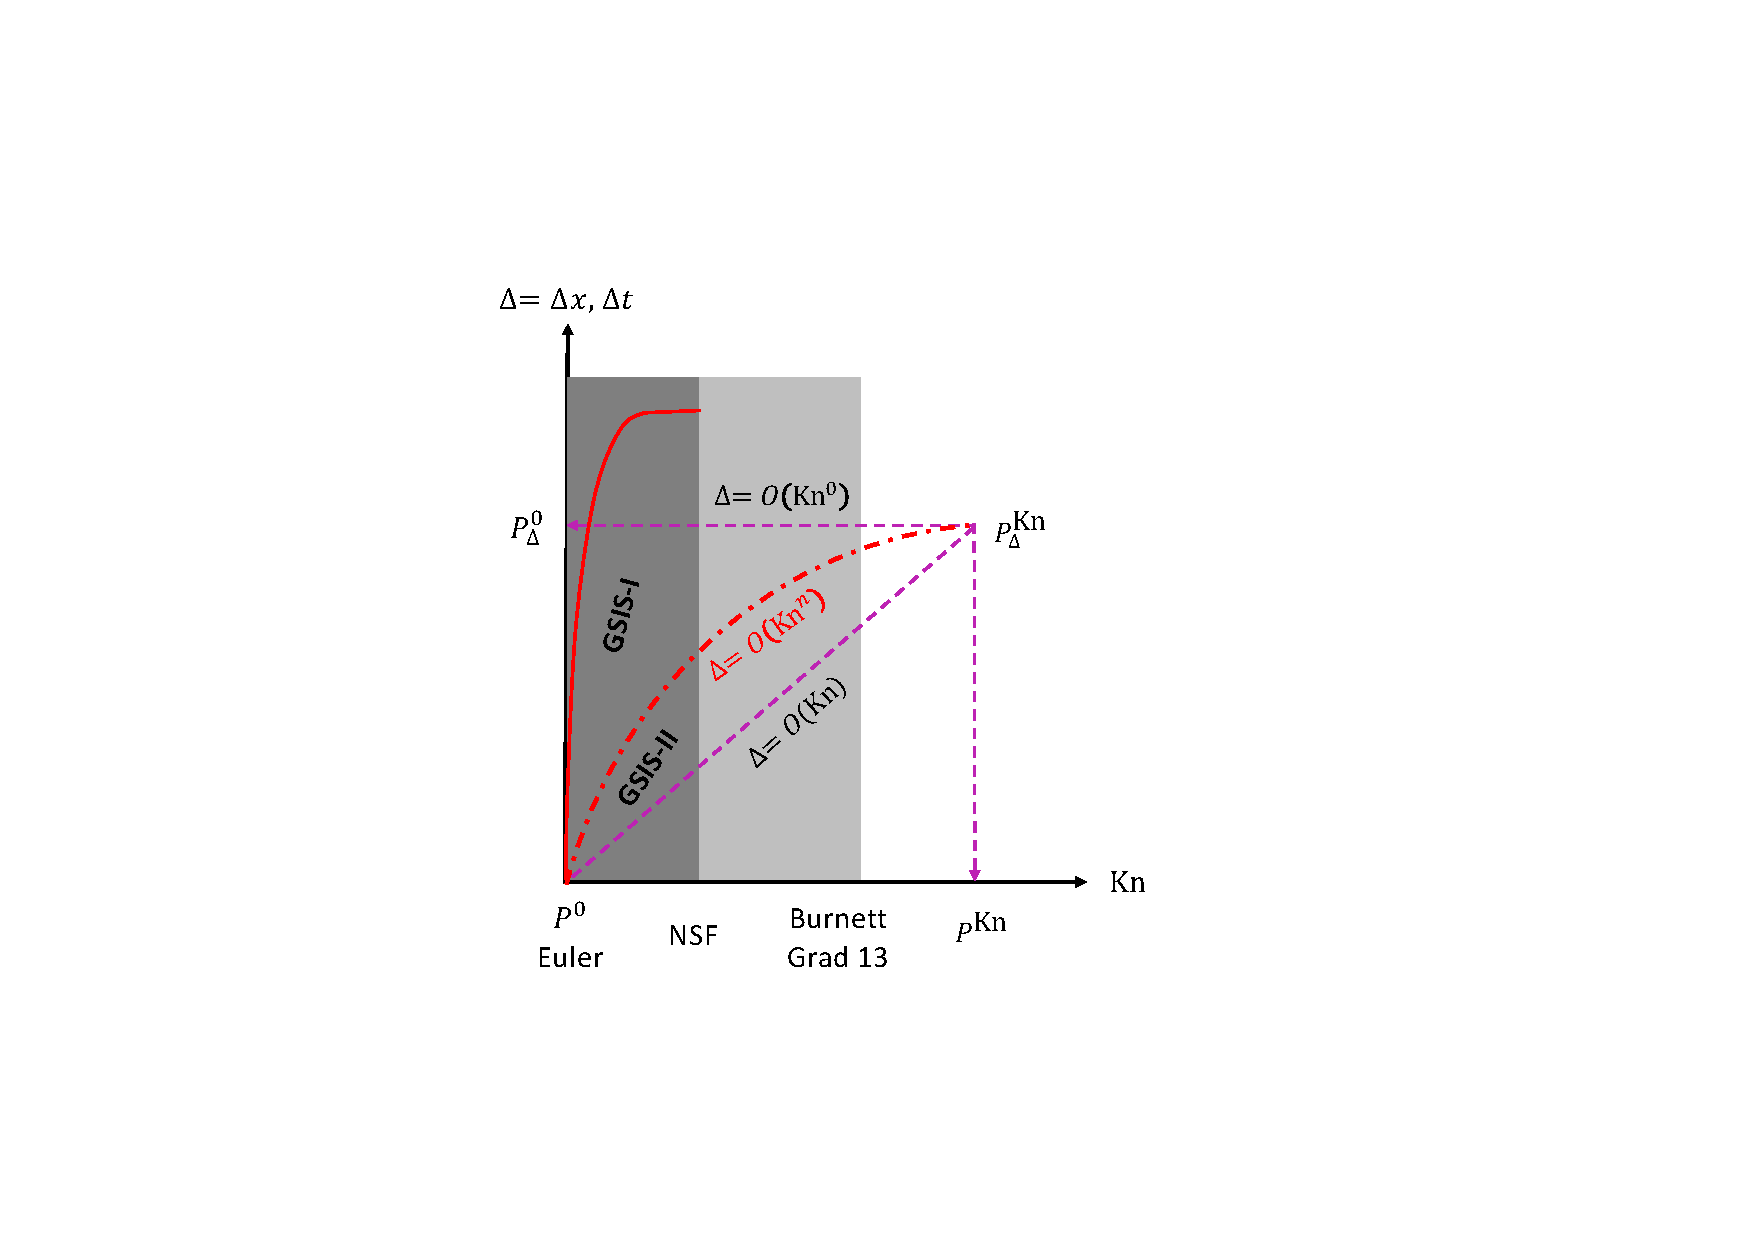
\includegraphics[scale=0.6]{GSIS_UP.pdf}
%	\caption{
%		Schematic of the asymptotic path to the limiting hydrodynamic flow regimes. The NSF equations are valid in the dark gray region. The region below the line $\Delta=O(\text{Kn})$ suggests resolved kinetic scale. The
%		red solid line stands for the maximum spatial grid size/time step to solve the NSF equations accurately using some discretization method (certainly $\Delta$ depends on the numerical method for NSF equations and specific flow problems; $\Delta$ could be larger than $O(1)$ because the time step can be proportional to $\text{Kn}^{-1}$ in some flows), below which GSIS-I can capture the hydrodynamic behavior. GSIS-II works at a smaller value of $\Delta$, say, beneath the dash-dotted line $\Delta=O(\text{Kn}^n)$. 
%	}
%	\label{fig:GSIS_UP}
%\end{figure}
%
%
%\subsection{Numerical results}\label{section_numerical}
%
%In this section we propose several numerical examples to assess the accuracy and efficiency of both GSIS schemes, as well as HOLO. 
%
%\subsubsection{Rayleigh-Brillouin scattering}\label{Osci_CRBS}
%
%The coherent Rayleigh-Brillouin scattering is a promising technique to probe the property of gas, in which the wavelike density perturbation in gas is created by a moving optical lattice. We choose this problem because it is a zero-dimensional problem so any one can quickly test/compare our and their methods. 
%
%Applying the Fourier transform in the scattering (say, $x_1$) direction, the governing equation for the velocity distribution function $h$ can be written as~\cite{Wu2020AIA}
%\begin{equation}\label{CRBS_LBE}
%\frac{\partial {h}}{\partial {t}}+2i\pi{}v_1h
%=\mathcal{L}(h)
%+2v_1\cos(2\pi{f_s}t)f_{eq},
%\end{equation}
%where $f_s$ is the frequency of the moving optical lattice; we choose $f_s=\sqrt{5/6}$ (i.e. the sound speed normalized by the most probable speed of gas molecules) so that the amplitude of perturbed density will scale as $1/\text{Kn}$ when the Knudsen number is small. If the numerical scheme cannot preserve the NSF limit when $\text{Kn}\rightarrow0$, then a very small time step is needed to keep a low numerical dissipation; otherwise the amplitude will be much smaller than the converged solution.  
%
%
%Since the spatial derivative $\partial/\partial{x_1}$ is replaced by $2i\pi$ in the Fourier transform, the conservation equations~\eqref{eq123} becomes
%\begin{equation}
%\begin{aligned}
%\frac{\partial{\varrho}}{\partial t}+2i\pi{{u}_1}=0, \\
%2\frac{\partial{u}_1}{\partial t}+2i\pi(\varrho+T+\sigma_{11})=2\cos(2\pi{f_s}t),\\
%\frac{3}{2}\frac{\partial{T}}{\partial t}+2i\pi(u_1+q_1)=0, 
%\end{aligned}
%\end{equation}
%and the same transform is applied to the synthetic equations for stress and heat flux in Eqs.~\eqref{sigma_HoT}, \eqref{q_HoT}, \eqref{HoT_sigma_TD}, and \eqref{HoT_q_TD}. 
%
%%while the shear stress and heat flux are modified into the following forms:
%%\begin{eqnarray}
%%\frac{\partial \sigma_{11}}{\partial t}+\text{HoT}_{\sigma_{11}}+\frac{8i\pi}{3}u_1=-\delta_\text{rp}\sigma_{11}, \label{sound_sigma} \\
%%\frac{\partial{q_1} }{\partial t}+\text{HoT}_{q_1}+\frac{5i\pi}{2}T=-\frac{2}{3}\delta_\text{rp}q_{1}. \label{sound_q}
%%\end{eqnarray}
%
%\begin{figure}[t]
%	\centering
%	\includegraphics[scale=0.35]{CRBS_delta1000.pdf}
%	\includegraphics[scale=0.35]{CRBS_delta1000BGK.pdf}
%	\caption{
%		The imaginary part of the density perturbation $\varrho$ in the coherent Rayleigh-Brillouin scattering, when the rarefaction parameter is $\delta_{rp}=1000$. Inset shows the iteration number, where the iteration is terminated when the relative error in macroscopic quantities between two consecutive iterations is less than $10^{-10}$. The kinetic equations are solved with a time step of $\Delta{t}=0.01$, by the backward Euler method and Crank-Nicolson scheme, respectively. The synthetic equations are always solved by the Crank-Nicolson scheme with the same time step.
%	}
%	\label{fig:CRBS}
%\end{figure}
%
%In the numerical simulation, the molecular velocity space $\bm{v}$ is discretized by $6\times6\times6$ Gauss-Hermite quadrature, which is accurate to resolve the velocity distribution function when the Knudsen number is small: in the continuum flow regime the velocity distribution function contains $v^3_i$, therefore, the integrand in the high order term in Eq.~\eqref{HoT_q_TD} has the highest polynomial of $v^7_i$, while the Gauss-Hermite quadrature of order 6 is accurate for polynomial up to the order of 11. Starting from the zero initial values for the velocity distribution function and macroscopic quantities, the synthetic equations are solved by the Crank-Nicolson scheme, while the kinetic equation is solved by backward Euler and Crank-Nicolson schemes, respectively. The inner iteration terminates when the relative error in density between two consecutive steps are less than $10^{-10}$. 
%
%
%
%
%It should be noted that in HOLO, in order to make the mesoscopic and macroscopic equations consistent, consistency terms are introduced to enslave the solution of synthetic equations to that of the kinetic equation~\cite{Taitano2014}. In this problem, since the spatial derivative is handled exactly by the Fourier transform, and the molecular velocity space is discretized by adequate quadrature, these consistency terms vanish. In GSIS, however, we enslave the solution of kinetic equation to that of the synthetic equations, since the kinetic equation converges so slowly that false convergence might happen~\cite{DSA2002,SuArXiv2019}. That is, when the inner iteration is converged (judged by the relative error in macroscopic quantities), the velocity distribution function is updated as per Eq.~\eqref{guided0} to reflect the converged macroscopic quantities.
%
%%\begin{equation}\label{correction}
%%\begin{aligned}[b]
%%h^{k+1}=h^{k+1/2}
%%&+ \left({\varrho}^{k+1}-\varrho^{k+1/2}\right)  +2\left({\bm{u}}^{k+1}-\bm{u}^{k+1/2}\right)\cdot\bm{v} \\
%%&+\left({T}^{k+1}-T^{k+1/2} \right) \left( v^2-\frac{3}{2} \right).
%%\end{aligned}
%%\end{equation}
%
%
%Numerical results of the GSIS and HOLO for coherent Rayleigh-Brillouin scattering is shown in Fig.~\ref{fig:CRBS}. From the figure we see that, when the kinetic equation is solved with second-order accuracy, GSIS-I, GSIS-II, and HOLO yield identical solutions. For the BGK model, in each time step, CIS needs around 200 inner iterations to find converged solutions (not shown), while GSIS-I, GSIS-II, and HOLO needs about 5 iterations. This is consistent with the Fourier stability analysis presented in Fig.~\ref{fig:GSIS12_time_dependent}, since the wavevector in this problem is always unity. For the Shakhov model, GSIS-I still needs 5 iterations, while GSIS-II and HOLO need about 20 iterations at each time step. This is because the former has synthetic equation for the evolution of heat flux that appears in the gain term of kinetic model so that the error decay rate approaches zero when $\text{Kn}\rightarrow0$, while the latter has the error decay rate approaching $1/3$. 
%
%
%We also find that, when the kinetic equation is solved with first-order temporal accuracy, both GSIS schemes yield accurate solutions. However, HOLO exhibits visible dissipation as the density amplitude is smaller. This is because the time step should be no larger than $O(\text{Kn})$ for first-order scheme, otherwise the artificial viscosity is comparable or larger than the physical viscosity, which leads to inaccurate solutions. It is very interesting to note that, if we turn off the correction of velocity distribution function in Eq.~\eqref{correction}, both GSIS schemes produce the same  inaccurate result as HOLO. This clearly demonstrates that we should enslave the solution of kinetic equation to that of the synthetic equation, while the HOLO does the reverse way and get inaccurate results.
%
%
%Finally, it should be noted that although GSIS-I allows a time step of $O(1)$ to asymptotic preserve the NSF limit, here it is chosen as $\Delta{t}=0.01$ because the NSF equations cannot be accurately solved by a second-order scheme when the time step is larger than 0.01 in this specific problem. 
%
%
%\begin{figure}[t]
%	\centering
%	\includegraphics[scale=0.5]{Vortex_t200delta1e4.pdf}
%	\caption{
%		Velocity profiles in the two-dimensional Taylor vortex flow at the time $t=200$, when the BGK model with $\delta_{rp}=10000$ is solved by GSIS. The profiles with time step $\Delta{t}=50$ are shifted upward for clarity. DVM 1st (2nd) order means that the kinetic equation is solved with first (second) order temporal accuracy.  Inset: velocity contour at $t=200$.
%	}
%	\label{fig:Taylor}
%\end{figure}
%
%\subsubsection{Decay of Taylor vortex}\label{Taylor_vortex}
%
%
%To test the property of fast converging and asymptotic NSF preserving of GSIS and HOLO at the time step $\Delta{t}\sim{O(1)}$, we consider the decay of  two-dimensional incompressible Taylor vortex within a periodic domain $0\le{x_1},x_2\le1$. In the continuum flow regime, the flow is governed by the incompressible Navier-Stokes equations and has the following analytical solution:
%\begin{equation}
%\begin{aligned}[b]
%u_1(x_1,x_2,t)=&-\cos(2\pi{x_1})\sin(2\pi{x_2})\exp\left(-{4\pi^2}t/{\delta_{rp}}\right),\\
%u_2(x_1,x_2,t)=&~~~\sin(2\pi{x_1})\cos(2\pi{x_2})\exp\left(-{4\pi^2}t/{\delta_{rp}}\right),
%\end{aligned}
%\end{equation}
%where the density and temperature are always zero. Therefore, the BGK model is used.
%
%
%
%This is an ideal test case to assess the asymptotic NSF preserving property, since when $\delta_{rp}$ is large ($\text{Kn}$ is small), the Taylor vortex takes a long time to decay, so the time step can be made very large if the numerical scheme for the kinetic system asymptotic preserves the NSF equations. 
%
%
%Without loss of generality we choose $\delta_{rp}=10^4$, and in order to focus only on the error in temporal discretization, we solve the kinetic equation and macroscopic synthetic equation by the Fourier spectral method in the spatial directions, with the spatial grid size of $\Delta{x}=1/16$. The kinetic equation is solved by the backward Euler and Crank-Nicolson scheme for the first- and second-order temporal accuracy, respectively, with the initial condition
%\begin{equation}
%h(\bm{v},t=0)=2[v_1u_1(x_1,x_2,0)+v_2u_2(x_1,x_2,0)]f_{eq},
%\end{equation}
%while the synthetic equations are solved by the second-order Crank-Nicolson scheme. The molecular velocity space $\bm{v}$ is discretized by $6\times6\times6$ Gauss-Hermite quadrature, which is sufficient accurate to evaluate the high order term in Eq.~\eqref{HoT_sigma_TD}.
%
%
%
%
%Numerical results are summarized in Fig.~\ref{fig:Taylor}. When $\Delta{t}=1$, both GSIS and HOLO yield accurate results (not shown for clarity). However, when $\Delta{t}$ is increased to 10, HOLO becomes unstable, which is consistent with the result from the Fourier stability analysis in Fig.~\ref{fig:GSIS12_time_dependent} (note that in this case the wavevector is $\theta=8\pi^2$).  Both GSIS schemes produce stable results, and converged solution in each time step is found within 4 iterations even when the time step is as large as $\Delta{t}=50$. From the figure one can also find that when the kinetic equation is solved with second-order temporal accuracy, accurate results are obtained. However, when the kinetic equation is solved with first-order temporal accuracy, GSIS-II generates inaccurate solutions when the time step is large, say, $\Delta{t}=50$. This is because GSIS-II do not have the property of asymptotic NSF preserving at large temporal step.
%
%To be specific, we find that in GSIS-II, when the streaming operator is treated exactly by the  Fourier spectral method, the first-order term in the Taylor expansion of velocity distribution function is given by Eq.~\eqref{h1_taylor}.
%% becomes
%%\begin{equation}
%%h^{(1)}=-\frac{\partial h^{(0)}}{\partial t_0}-\bm{v}\cdot\frac{\partial{h^{(0)}}}{\partial\bm{x}}-O(\Delta{t}^m)\delta_t(h).
%%\end{equation}
%Suppose $\Delta{t}\sim{O(1)}$, it is estimated that the last error term has a contribution to the shear viscosity at the order of 
%\begin{equation}
%\Delta{t}\left(\frac{4\pi^2}{\delta_{rp}}\right)^{m+1}
%=\underbrace{\left(\Delta{t}\frac{16\pi^4}{\delta_{rp}}\right)}_{O(1)}
%\left(\frac{4\pi^2}{\delta_{rp}}\right)^{m-1}
%\frac{1}{\delta_{rp}},
%\end{equation}
%where the underbraced term can be made $O(1)$ since this is largest time step to get the Navier-Stokes equation correct when solved by the second-order temporal scheme.
%Therefore, when the kinetic equation is solved by the backward Euler scheme, we have $m=1$ and the error term is at  the same order with the viscosity coefficient, hence the GSIS-II is not accurate at large time step. However, when the kinetic equation is solved by the second-order temporal accuracy, we have $m=2$. Therefore, the error term is much smaller than the viscosity coefficient when the Knudsen number is small. In this case, GSIS-II can yield accurate NSF solutions even at large time steps, as observed in Fig.~\ref{fig:Taylor}.
%
%
%% \footnote{Actually the velocity amplitude is governed by the following equation: $\frac{\partial u}{\partial t}=-\frac{4\pi^2}{\delta_{rp}}u$. }. 
%
%\begin{figure}[t]
%	\centering
%	\includegraphics[scale=0.4]{OscillatingCouette_delta1000T60omega0_1.pdf}
%	\caption{
%		Velocity profiles in the oscillating Couette flow at the time $t=60$, when the BGK model with $\delta_{rp}=1000$ is solved by the two GSIS schemes with different spatial resolution, with the time step $\Delta{t}=1$. The reference solution is obtained from GSIS-I with $N=121$ and $\Delta{t}=0.1$. Both kinetic and synthetic equations are solved by the Crank-Nicolson scheme. Inset: the inner iteration number at each time step.  
%	}
%	\label{fig:Couette}
%\end{figure}
%
%\subsubsection{Oscillatory Couette flow}\label{Osci_Couette}
%
%Consider the oscillatory Couette flow between two parallel plates and investigate the combined effect of spatial and temporal discretizations. The plate located at $x_1=0$ oscillates in the $x_2$ direction with the velocity
%\begin{equation}
%u_{wall}=\sin(2\pi{f_s}t),
%\end{equation}
%while the other plate at $x_1=1$ is stationary. The rarefaction parameter is chosen to be $\delta_{rp}=1000$, while the oscillation frequency is $2\pi{f_s}=0.1$. This problem can be greatly simplified. In fact, we have $\rho=T=0$, and the only the evolution equations for the velocity $u_2$ and stress $\sigma_{12}$ are needed. 
%
%
%
%
%
%%This problem can be greatly simplified. In fact, we have $\rho=T=0$, and the velocity is governed by
%%\begin{equation}
%%\begin{aligned}
%%2\frac{\partial {u_2}}{\partial{t}}
%%+\frac{\partial {{\sigma_{12}}}}{\partial{x_1}}=0, 
%%\end{aligned}
%%\end{equation}
%%and in GSIS-I the evolution equation for stress is
%%\begin{equation}
%%\begin{aligned}[c]
%%\frac{\partial \sigma_{12}}{\partial {t}}
%%+2\int{\left(v_1^2-\frac{1}{2}\right)v_2} \frac{\partial h}{\partial x_1}d\bm{v}
%%+\frac{\partial{u_2}}{\partial {x_1}}=-\delta_{rp}\sigma_{12}.
%%\end{aligned}
%%\end{equation}
%
%
%
%
%The spatial coordinate $x_1\in[0,1]$ is discretized non-uniformly with $N$ points, in the following manner
%\begin{equation}\label{spatial_discretization}
%x_1=\frac{1}{2}+\frac{\tanh(8m)}{2\tanh(4)}, \quad
%j=\frac{0,1,\cdots,N-1}{N-1}-\frac{1}{2},
%\end{equation}
%so that the Knudsen layer can be well resolved. Later it will be shown this affects the efficiency of inner iterations.  The molecular velocity space $v_2\times{v_3}$ is discretized by $6\times6$ Gauss-Hermite quadrature, while $v_1$ is discretized non-uniformly as per Eq.~\eqref{nonuniform_v} with $N_v=32$. 
%
%
%The kinetic equation is solved by the Crank-Nicolson scheme with second-order spatial and temporal accuracy, with the initial condition $h(x_1,\bm{v},t=0)=0$, and the boundary conditions are $h(x_1=0,v)=2u_{wall}v_2f_{eq}$ for $v_1>0$  and $h(x_1=1,v)=0$ for $v_1<0$.
%%\begin{equation}
%%\left\{
%%\begin{array}{lll}
%%h(x_1=0,v)=2u_{wall}v_2f_{eq}, & v_1>0,\\
%%h(x_1=1,v)=0, & v_1<0.
%%\end{array}
%%\right.
%%\end{equation}
%The synthetic equations are solved by the second-order temporal accuracy, while the spatial derivative is approximated by central finite-difference with 5 stencils; hence in the solving the synthetic equations $j$ in Eq.~\eqref{spatial_discretization} is taken from 2 to $N-3$, while the 4 left points, obtained from the kinetic equation, provide boundary conditions to synthetic equations. 
%
%
%%For wall-bounded problems, the boundary condition should be provided. For the kinetic equation we have
%
%%While for the synthetic equation, the boundary condition is provided from that from the kinetic equation. 
%
%
%
%
%
%\begin{figure}[t]
%	\centering
%	\includegraphics[scale=0.55]{HOLO.pdf}
%	\caption{
%		The error decay rate as a function of the rarefaction parameter in GSIS and HOLO. For wall bounded problems such as the Poiseuille and Couette flows, the perturbation from the wall bears a wavevector of $|\bm{\theta}|=\delta_{rp}$ if the Knudsen layer is resolved. Therefore, HOLO is only stable when the time step is small, while the robustness of two GSISs is manifested at any time step.
%	}
%	\label{fig:HOLO_time_dependent}
%\end{figure}
%
%
%Numerical solutions of the oscillatory flow at $\delta_{rp}=1000$ are shown in Fig.~\ref{fig:Couette} for different spatial resolutions. It is seen that when the number of spatial grid is decreased from  $N=121$ to 61 and then to 21, the accuracy of GSIS-I barely reduces. However, in GSIS-II when $N=21$, large difference to the reference solution is observed. This is for the GSIS-II the NSF equations can only be derived exactly when the spatial resolution is about $\Delta{x}={O(\sqrt{\text{Kn}})}\approx0.032$. When $N=121, 61$, and 21, the maximum grid size according to Eq.~\eqref{spatial_discretization} are 0.033, 0.066, and 0.190, respectively. The case of $\max(\Delta{x})=0.190$ is certainly too large. 
%
%
%On the other hand, we find that, when the same spatial resolution is used, generally speaking, GSIS-I needs less iteration numbers than GSIS-II. When $N$ is decreased, the iteration number increases. This is because this flow is driven by the oscillation of left plate; smaller value of $N$ means coarser spatial grid size and hence the information from the plate cannot be effectively passed to the bulk flow regime. Therefore, the use of non-uniform spatial grid~\eqref{spatial_discretization} not only allows the capture of flow dynamics around the Knudsen layer, but also facilitates fast convergence.
%
%
%\begin{figure}[t]
%	\centering
%	\includegraphics[width=0.45\textwidth]{OscillatingCouette_delta1000T60omega0_1Y015.pdf}
%	\includegraphics[width=0.45\textwidth]{OscillatingCouette_delta1000T60omega0_1Y05.pdf}
%	\caption{
%		Velocity profiles in the oscillating Couette flow at $x_1=0.15$ and 0.5, when the BGK model with $\delta_{rp}=1000$ is solved by GSIS-I with $\Delta{t}=5$ and 10, respectively. The reference solution is obtained from GSIS-I with  $\Delta{t}=0.1$. Both kinetic and synthetic equations are solved by the Crank-Nicolson scheme, when the spatial region is discretized by Eq.~\eqref{spatial_discretization} with $N=121$.   
%	}
%	\label{fig:Couette_time}
%\end{figure}
%
%
%
%Note that the result of HOLO is not shown, since we find that it is not stable when $\Delta{t}>0.004$. This can be understood as follows. When the Knudsen layer is resolved, the oscillating plate will generate a perturbation with a wavelength at the order of MFP, that is, the wavevector is 
%\begin{equation}
%\theta\approx2\pi\delta_{rp}.
%\end{equation} 
%With this information, we re-calculate the error decay rate of GSIS-I, GSIS-II and HOLO in Fig.~\ref{fig:HOLO_time_dependent} with $\theta=\delta_{rp}$. It is seen that GSIS is stable, while HOLO is unstable when $\Delta{t}>0.01$ at $\delta_{rp}=1000$. This is consistent with our numerical observations. If a coarse spatial grid is used, the stability region of HOLO increases, however, the convergence speed is much reduced.  
%
%
%We also assess the temporal accuracy of GSIS-I. It is seen from Fig.~\ref{fig:Couette_time} that even when the time step is much large than the mean collision time of gas molecules, say, one sixth of the oscillation frequency, the phase of the velocity is preserved after 10 oscillation periods. 
%
%%HOLO is not stable because around the Knudsen layer the effective Knudsen number is around 1, and the perturbation wavevector is about $\Delta{x}\sim\delta_{rp}$, therefore, according to Fig.~\ref{fig:GSIS12_time_dependent} the maximum time step for stable iteration is about $10/\delta_{rp}$.
%
%%GSIS-I and GSIS-II need roughly the same iteration number because the effective Knudsen number is around 1, therefore
%
%
%%
%%\section{Nonlinear GSIS}
%%
%%We apply the GSIS with Scheme II to find the stationary solution of the supersonic rarefied gas flow passing a circular cylinder. The 2D flow domain is an annulus with the inner circle with radius $r_\text{in}$ being the cylinder surface, and the outer circle with radius of $r_\text{out} = 11r_\text{in} $ being the far-field boundary. The free-stream Mach number is $\text{Ma}_{\infty}$. The cylinder surface temperature is set as the same as the free-stream temperature $T_\text{w} = T_\infty$. To properly compare with the reported results~\cite{zhuDiscreteUnifiedGas2016,zhuyajun2016}, the Knudsen number is defined as
%%\begin{equation}
%%\text{Kn} = \frac{(5-2\omega)(7-2\omega)\mu v_m}{15\sqrt{\pi}p r_\text{in}}
%%\end{equation}
%%where $\mu$, $v_m$ and $p$ are the viscosity, most probable molecular velocity and pressure at the free-stream condition, respectively. Detailed numerical method and parameter settings are given in Ref.~\cite{Zhu2021JCP}.
%%%Note that such a definition of Kn is different from the one in the previous cases of this article.
%
%
%%Due to symmetry, only the upper-half domain is computed and the symmetric boundary condition is applied. The physical grid size is $M\times N$, where $M$ is the number of cells along the upper surface of the cylinder and $N$ is the number of cells along the radial direction. The cell height along the radial direction grows with a constant expansion ratio from the first layer's height ($\Delta r_\text{min}$). The cell width along the cylinder surface grows from leading and trailing edges of the cylinder toward the upper position with a constant expansion ratio, such that the largest cell's width is five times of the smallest one. For the cases of Kn = 1 and 0.1, the physical grid is set as $N = 50$, $M = 64$ and $\Delta r_\text{min} = 0.01$, while for the case of Kn = 0.01, $N=80$, $M=80$ and $\Delta r_\text{min} = 0.001$. The discrete velocity set is a uniform Cartesian grid with $90^2$ points in the range of $[-15,15]^2$. \leir{The DVM method is implemented using the implicit time-stepping scheme as described in Sec.~\ref{sec:dvm2}. The CFL number in the DVM and NS solvers are 1000 and 100, respectively. The convergence criterion of the outer loop and inner loop in Eq.~\eqref{convtol} are set as $\epsilon_{\text{out}} = {1e-6}$ and $\epsilon_{\text{in}} = {1e-6}$. }
%
%
%%\begin{figure}[t]
%%	\centering
%%	%	\includegraphics[width=0.45\textwidth]{T_a787_f548.pdf}
%%	%	\includegraphics[width=0.45\textwidth]{Ma_a787_f548.pdf} \\
%%	\includegraphics[width=0.45\textwidth]{T_9cae_cb30.pdf}
%%	\includegraphics[width=0.45\textwidth]{Ma_9cae_cb30.pdf}\\
%%	\includegraphics[width=0.45\textwidth]{T_7d6d_1f2d.pdf}
%%	\includegraphics[width=0.45\textwidth]{Ma_7d6d_1f2d.pdf}
%%	\caption{Cylinder flow at $\text{Ma}_\infty$ = 5 and (top)  $\text{Kn=0.1}$ and (bottom) $\text{Kn=0.01}$: comparison of the non-dimensional temperature (left) and local Mach number (right) fields obtained by CIS and GSIS, together with the reference discrete-UGKS and DSMC solutions extracted from Ref.~\cite{zhuyajun2016}. GSIS results: colored background with white solid lines; CIS solutions: dashed yellow lines. The discrete-UGKS and DSMC solutions are represented by the solid red lines and dashed black lines, respectively.}% \zhu{a787 vs f548}
%%	\label{fig:cylinder_Kn1}
%%\end{figure}
%
%%Fig.~\ref{fig:cylinder_Kn1} presents the temperature and local Mach number contour of the results predicted by GSIS and CIS, which are overlapped with the literature results wherever available, in particular the DSMC and discrete-UGKS solution~\cite{zhuDiscreteUnifiedGas2016}. We can observe good agreement between the CIS and GSIS solutions, and overall good matches with the results reported in literature. %Fig.~\ref{fig:cylinder_Kn1_surface}  shows the pressure (normal stress), shear stress and heat flux along the upper surface of the cylinder. Comparisons are made with the results from the literature including Refs.~\cite{zhuDiscreteUnifiedGas2016} and \cite{zhuImplicitUnifiedGaskinetic2016}. Again, it is shown that current GSIS results agree well with the reported results. 
%
%%To assess the efficiency of GSIS, we plot the convergence history of the DVM steps in both GSIS and CIS in Fig.~\ref{fig:cylinder_convergence}. In addition, 
%
%%Table~\ref{tab:cyliner_time} lists the number of DVM steps and overall computing time in the same environment as in the lid-driven cavity flow. Obviously, for highly rarefied flows,  CIS is very efficient: when Kn = 1, the solution converges after 186 steps and the total computing time is around 12 minutes. For this case, GSIS needs more DVM steps than the CIS, and the overall computing time is about twice of CIS. As Kn decreases to 0.1, GSIS becomes slightly more efficient than CIS. When Kn = 0.01,  CIS requires as many as 4925 DVM steps and needs around 8 hours to reach convergence, while GSIS takes only 42 minutes and converges within 210 DVM steps. %We note that for small-Kn cases, the inner loop solving the synthetic equations also takes much fewer time steps to converge, because in these case the Reynolds numbers are much higher, favoring a fast convergence of the NSF solver. 
%
%%\begin{figure}[t]
%%	\centering
%%	\includegraphics[width=0.5\textwidth]{cylinder_conv_compare_annoted.pdf}
%%	\caption{Convergence history of the DVM time stepping in the supersonic cylinder flow at different Knudsen number. The red, green and blue lines are for Kn = 1, 0.1 and 0.01, respectively. The solid and dashed lines represent the CIS and GSIS results, respectively.}
%%	\label{fig:cylinder_convergence}
%%\end{figure}
%
%%%NOTE: convtol all 4 vars < 1e-6, actually the 3rd one converges lastly
%%\begin{table}[t]
%%	\centering
%%	\caption{Number of DVM steps in CIS and GSIS and the overall CPU time for the supersonic cylinder flow.}
%%	\begin{tabular}{rrrrrrr}
%%		\toprule
%%		\multicolumn{1}{l}{Kn} & \multicolumn{1}{r}{Physical} & \multicolumn{1}{r}{Velocity} &\multicolumn{1}{r}{CIS: DVM} & CIS: CPU & \multicolumn{1}{r}{GSIS: DVM} & GSIS: CPU \\
%%		\multicolumn{1}{r}{} & \multicolumn{1}{r}{grid size} & \multicolumn{1}{r}{grid size} &\multicolumn{1}{r}{steps} &\multicolumn{1}{r}{time} & \multicolumn{1}{r}{steps}& \multicolumn{1}{r}{time} \\
%%		\midrule
%%		
%%		$1$   & $64\times 50$ &  $90\times 90$ & $186$    & $ 12$ min & 264  & $27 $ min \\
%%		$0.1$  & $64\times 50$ &  $90\times 90$  & $552$    & $ 36$ min & 232  & $ 24 $ min \\
%%		$0.01$ & $80\times 80$ & $90\times 90$ & $4,925$  & $508$ min & 210  & $42$ min \\
%%		\bottomrule
%%	\end{tabular}%
%%	\label{tab:cyliner_time}%
%%\end{table}%
%
%
%








\section{Concluding remarks and Outlooks}\label{sec:summary}

Various numerical results have demonstrated that GSIS is able to find the converged solution within dozens of iterations at any Knudsen number, even when the spatial cell size is much larger than the MFP in the bulk flow region. Moreover, the fast converging property of GSIS enables the numerical error decay fast and the convergence criterion can be set at a much higher value than the CIS. 

In addition to the fast-converging and asymptotic-persevering properties that have been prove rigorously,  GSIS has the following advantages:
\begin{enumerate}	
	\index{unified gas kinetic scheme}
	
	%\item Compared to the implicit UGKS~\cite{zhuyajun2016} and it variants~\cite{yang2018PoF,yang2018PRE}, as well as the high-order-low-order scheme~\cite{Taitano2014}, we conclude that in order to develop efficient multiscale numerical schemes, macroscopic equations must be solved together with the Boltzmann or kinetic model equations. While in Refs.~\cite{zhuyajun2016,yang2018PoF,yang2018PRE} only five equations from the conservation laws are used so that complex flux evaluation across the cell interface must be adopted to asymptotically preserve the Navier-Stokes limit, GSIS needs no flux evaluation as the NSF equations are recovered explicitly. Thus, the numerical implementation of GSIS is much easy than UGKS and the convergence to steady-state solution is much faster. More importantly, our scheme does not depend on the specific form of the collision operator, while that in Refs.~\cite{zhuyajun2016,yang2018PoF,yang2018PRE} relies only on the BGK-type kinetic equations to enable exact evaluation of numerical flux. 
	
	\item \textbf{Compatibility with CFD techniques.} The gas kinetic equation and synthetic equations can be solved by sophisticated methods in computational fluid dynamics, and the kinetic and macroscopic solvers can have different orders of accuracy. For highly rarefied gas flows, the spatial cell size is usually smaller than the MFP and both methods yield high accuracy. For continuum/or near continuum flows, as long as the macroscopic solver for synthetic equations (which are essentially the NSF equations) is able to capture the continuum flow behaviors, the accuracy of GSIS is guaranteed, that is, the numerical cell size can be much larger than the MFP, but should be smaller than the variation scale (such as the sound wavelength) of the flow. %In other words, the solution of GSIS is not affected when gas kinetic equation and synthetic equations are discretized by different schemes, as long as synthetic equation captures the flow dynamics in the continuum regime. %For example, in the 2D thermal edge flow, the gas kinetic equation is solved by DG with different order of accuracy.   
	
	\item  \textbf{Universality.}  GSIS can be easily extended to nonlinear flows, time-dependent systems, and rarefied flow of polyatomic gas~\cite{Zhu2021JCP,Su2021CMAME}. Extension to DSMC (to remove the limitation on cell size and boost convergence) is also possible, since the GSIS relies on no specific collision operator so that it can be extended naturally to multi-species flows and even flows involving chemical reactions. 
%	GSIS may be applied to low-variance~\cite{Radtke2009PRE,Radtke2011} and even frequency-domain~\cite{Ladiges2015JCP} DSMC that solves the linearized Boltzmann and kinetic model equations to improve the computational efficiency, especially in the near-continuum flow regime. 
	
\end{enumerate}  


With these development implemented, it is hoped that the multiscale simulation of rarefied gas flows is solved completely in the near future. Also, the essential idea is ready to be applied to other kinetic equations such as the Enskog equation for dense gases with applications to gas extraction in unconventional reservoirs and non-equilibrium evaporation and condensation at the nanoscale~\cite{Lei2015Enskog,Wu2016JFM}, as well as the Callaway model on nonequilibrium phonon transport with dual relaxation times~\cite{Liu2021Callway}.






%\appendix
%
%\section*{Appendix}
%\renewcommand{\theequation}{A.\arabic{equation}}
%
%Here, some details to solve the synthetic equations using the high-order hybridizable discontinuous Galerkin (HDG) method~\cite{Cockburn2010} on arbitrary triangular mesh are presented. The steady-state governing equations can be written in the following mixed form as a system of first-order equations
%\begin{equation}
%\begin{aligned}[b]
%\nabla\cdot\left[\bm{\mathcal{G}}_\text{c}+\bm{\mathcal{G}}_\text{d}\right]=0,\\
%\bm{L}-\nabla\bm u-\bm{\Pi}=0,\\
%\bm{E}-\nabla T-\bm{\Theta}=0,
%\end{aligned}
%\end{equation}
%where
%\begin{equation}
%\begin{aligned}[b]
%\bm{\mathcal{G}_\text{c}}=\left[\begin{array}{c}
%\bm U\\p\bm I\\\bm 0
%\end{array}
%\right],\\
%\bm{\mathcal{G}_\text{d}}=\left[\begin{array}{c}
%\bm 0\\-\frac{1}{\delta_{rp}}\left(\bm L+\bm L^{\text{T}}-\frac{2}{3}\mathrm{tr}\left(\bm L\right)\bm I\right)\\
%-\frac{5}{4\delta_{rp}\mathrm{Pr}}\bm E
%\end{array}
%\right],\\
%\bm{\Pi}=\left[\begin{array}{cc}
%\text{HoT}_{\sigma_{11}}+\frac{1}{2}\text{HoT}_{\sigma_{22}} & \frac{1}{2}\text{HoT}_{\sigma_{12}}\\
%\frac{1}{2}\text{HoT}_{\sigma_{12}} & \frac{1}{2}\text{HoT}_{\sigma_{11}}+\text{HoT}_{\sigma_{22}}
%\end{array}
%\right],\\
%\bm{\Theta}=\left[\begin{array}{c}
%\frac{4}{5}\text{HoT}_{q_{1}} \\
%\frac{4}{5}\text{HoT}_{q_{2}} 
%\end{array}
%\right],
%\end{aligned}
%\end{equation}
%with $\bm{I}$ being the identity matrix. The auxiliary variables $\bm{L}$ and $\bm{E}$ are introduced to approximate the combination of the velocity gradient $\nabla\bm{u}$, temperature gradient $\nabla T$ and the high-order moments. Then, the stress tensor and heat flux are evaluated as
%\begin{equation}\label{sq}
%\sigma_{ij}=-\frac{1}{\delta_{rp}}\left(L_{ij}+L_{ji}-\frac{2}{3}L_{kk}\delta_{ij}\right),\quad q_i=-\frac{5}{4\delta_{rp}\mathrm{Pr}}E_i.
%\end{equation}
%
%Let $\Delta\in\mathbb{R}^2$ be an two-dimensional domain with boundary $\partial\Delta$ in the $x_1-x_2$ plane. Then, $\Delta$ is partitioned in $M$ disjoint regular triangles $\Delta_i$: $\Delta=\cup^{M}_i\Delta_i$. The boundaries $\partial\Delta_i$ of the triangles define a group of $N$ faces $\Gamma_c$: $\Gamma=\cup^{M}_i\{\partial\Delta_i\}=\cup^{N}_c\{\Gamma_c\}$. For HDG discretization, two types of discontinuous finite element approximation space, one for solutions within $\Delta_i$ and the other for traces of solution on $\Gamma_c$, are defined as
%\begin{equation}
%\begin{aligned}[b]
%\mathcal{V}=\{\varphi:\ \varphi|_{\Delta_i}\in\mathcal{P}^k(\Delta_i),\ \forall\ \Delta_i\subset\Delta\},\\
%\mathcal{W}=\{\psi:\ \psi|_{\Gamma_c}\in\mathcal{P}^k(\Gamma_c),\ \forall\ \Gamma_c\subset\Gamma\},
%\end{aligned}
%\end{equation}
%where $\mathcal{P}^k(D)$ denotes the space of $k-$th order polynomials on a domain $D$. 
%
%
%The HDG method solves the system in two steps. First, a global problem is set up to determine the traces of the flow properties $\hat{\bm{Q}}=\left[\hat{p},\hat{\bm{u}},\hat{T}\right]$ on the faces $\Gamma$. Then, a local problem with $\hat{\bm{Q}}$ as the boundary condition on $\partial\Delta_i$ is solved element-by-element to obtain the solutions for the flow properties $\bm{Q}=\left[p,\bm{Q},T\right]$, as well as the ones for the auxiliary variables $\bm{L}$ and $\bm{E}$. Generally speaking, when moving from the interior of the triangle element $\Delta_i$ to its boundary $\partial\Delta_i$, the traces defines what the values of field variables on the boundary should be. In the HDG method, it is assumed that the traces are singled-valued on each face. 
%
%We introduce the notations $\left(a,b\right)_D=\int_{D\in\mathbb{R}^2}\left(a\odot b\right)\mathrm{d}x_1\mathrm{d}x_2$ and $\langle a,b\rangle_D=\int_{D\in\mathbb{R}^1}\left(a\odot b\right)\mathrm{d}\Gamma$, where $\odot$ can be either the dot product $\cdot$ or tensor product $\otimes$. The local problem is stated as: find $\left(\bm{Q},\bm{L},\bm{E}\right)\in\left[\mathcal{V}\right]^4\times\left[\mathcal{V}\right]^4\times\left[\mathcal{V}\right]^2$ such that
%\begin{equation}\label{local}
%\begin{aligned}[b]
%-\left(\bm{\mathcal{G}_\text{c}}+\bm{\mathcal{G}_\text{d}},\nabla\bm{r}\right)_{\Delta_i}+\langle\hat{\bm{\mathcal{F}}}\cdot\bm{n},\bm{r}\rangle_{\partial\Delta_i}=0,\\
%\left(\bm{L},\bm{w}\right)_{\Delta_i}+\left(\bm{u},\nabla\cdot\bm{w}\right)_{\Delta_i}-\langle\hat{\bm{u}},\bm{w}\cdot\bm{n}\rangle_{\partial\Delta_i}=\left(\bm{w},\bm{\Pi}\right)_{\Delta_i},\\
%\left(\bm{E},\bm{z}\right)_{\Delta_i}+\left(T,\nabla\cdot\bm{z}\right)_{\Delta_i}-\langle\hat{T},\bm{z}\cdot\bm{n}\rangle_{\partial\Delta_i}=\left(\bm{z},\bm{\Theta}\right)_{\Delta_i},
%\end{aligned}
%\end{equation}  
%for all $\left(\bm{r},\bm{w},\bm{z}\right)\in\left[\mathcal{V}\right]^4\times\left[\mathcal{V}\right]^4\times\left[\mathcal{V}\right]^2$. The numerical flux $\hat{\bm{\mathcal{F}}}\cdot\bm{n}$ is defined as~\cite{Peraire2010}
%\begin{equation}
%\hat{\bm{\mathcal{F}}}\cdot\bm{n}=\left[\begin{array}{c}
%\bm{u}\\
%\hat{p}\bm{I}-\frac{1}{\delta_{rp}}\left(\bm{L}+\bm{L}^{\mathrm{T}}-\frac{2}{3}\mathrm{tr}\left(\bm L\right)\bm{I}\right)\\
%-\frac{5}{4\delta_{rp}\mathrm{Pr}}\bm{E}
%\end{array}\right]\cdot\bm{n}+\left[\begin{array}{ccc}
%\tau & &\\
%& \frac{\tau}{\delta_{rp}} &\\
%& & \frac{5\tau}{4\delta_{rp}\mathrm{Pr}}
%\end{array}
%\right]\left[\begin{array}{c}
%p-\hat{p}\\
%\bm{u}-\hat{\bm U}\\
%T-\hat{T}
%\end{array}\right].
%\end{equation}
%Here $\bm{n}$ being the outward unite normal vector of $\partial\Delta_i$. $\tau$ is the stabilization parameter that have important effects on the accuracy and convergence of the HDG method. In this work, we chosen $\tau=1/H_\text{min}$, with $H_\text{min}$ the minimum height of the triangles $\Delta_i$. 
%
%The global problem is set up by enforcing the continuity of the numerical flux over all the interior faces. It is stated as: find $\hat{\bm{Q}}\in\left[\mathcal{W}\right]^4$ such that
%\begin{equation}\label{Global1}
%\langle\bm{\left(\hat{\mathcal{F}}}\cdot\bm{n}\right)^+,\bm{\psi}\rangle_{\Gamma_c}+\langle\bm{\left(\hat{\mathcal{F}}}\cdot\bm{n}\right)^-,\bm{\psi}\rangle_{\Gamma_c}=0,\quad\text{on}\ \Gamma_c\in\Gamma\backslash\partial\Delta,
%\end{equation}
%for all $\bm{\psi}\in\left[\mathcal{W}\right]^4$. Here the superscripts $\pm$ denote the numerical fluxes obtained from the triangles on both sides of the face. Note that the traces on boundary faces are calculated as
%\begin{equation}\label{Global2}
%\langle\hat{\bm Q}-\bm{Q}^+_{VDF},\bm{\psi}\rangle_{\Gamma_c},\quad\text{on}\ \Gamma_c\in\Gamma\cap\partial\Delta,
%\end{equation}
%where $\bm{Q}^+_{VDF}$ is the field solutions directly calculated from the approximated VDF (see Eq.~\eqref{MP}) within the triangle where the boundary face $\Gamma_c$ belongs to. 
%
%By assembling the local problem~\eqref{local} and global problem~\eqref{Global1} and~\eqref{Global2} over all the triangles and faces, we can obtain a matrix system of form
%\begin{equation}
%\left[\begin{array}{cccc}
%A_Q & A_L & A_E & A_{\hat{Q}}\\
%B_Q & B_L & B_E & B_{\hat{Q}}\\
%C_Q & C_L & C_E & C_{\hat{Q}}\\
%D_Q & D_L & D_E & D_{\hat{Q}}\\
%\end{array}
%\right]\left[\begin{array}{c}
%\mathbb{Q}\\
%\mathbb{L}\\
%\mathbb{E}\\
%\hat{\mathbb{Q}}
%\end{array}
%\right]=\left[\begin{array}{c}
%S_{Q}\\
%S_{L}\\
%S_{E}\\
%S_{\hat{Q}}
%\end{array}
%\right],
%\end{equation}
%where $\mathbb{Q}$, $\mathbb{L}$, $\mathbb{E}$ and $\hat{\mathbb{Q}}$ are the vectors of degrees of freedom of the flow properties $\bm{Q}$, the auxiliary variables $\bm{L}$ and $\bm{E}$, and the trace of the flow properties $\hat{\bm{Q}}$, respectively. Note that the degrees of freedom for $\bm{Q}$, $\bm{L}$ and $\bm{E}$ are grouped together and ordered element-by-element, and the corresponding coefficient matrix $\left[A_Q,A_L,A_E;B_Q,B_L,B_E;C_Q,C_L,C_E\right]$ has block-diagonal structure. Therefore, we can eliminate $\bm{Q}$, $\bm{L}$ and $\bm{E}$ to obtained a reduced linear system involving only $\hat{\mathbb{Q}}$. Once $\hat{\mathbb{Q}}$ is determined, $\bm{Q}$, $\bm{L}$ and $\bm{E}$ are reconstructed corresponding to the local problem~\eqref{local} in an element-wise fashion, while the stress tensor and heat flux are calculated as Eq.~\eqref{sq}.

    


